\documentclass[11pt,a4paper]{article}

% USEPACKAGE LISTA
\usepackage[utf8]{inputenc}
\usepackage{amsmath}
\usepackage{mathtools}
\usepackage{marvosym} 
\usepackage{wrapfig}
\usepackage{hyperref}
\usepackage{float}
\usepackage{multicol}
\hypersetup{colorlinks,citecolor=black,filecolor=black,linkcolor=black,urlcolor=black}
\usepackage{pdfpages}
\usepackage{amsfonts}
\usepackage{amssymb}
\usepackage{fancyhdr}
\usepackage{graphicx}
\usepackage{t1enc}
\usepackage[magyar]{babel}
\usepackage{bm}
\usepackage{tikz, tcolorbox}
\usepackage{fancyvrb}
\usepackage{subfigure}
\usepackage{subcaption}
\usepackage[export]{adjustbox}

\usepackage{pgfplots}
\pgfplotsset{height = 10cm, width=15cm,compat=1.9}

% \usepackage[usenames,dvipsnames]{xcolor}
\usepackage[left=2cm,right=2cm,top=2cm,bottom=2cm]{geometry}

\setlength{\parindent}{0pt}
\setlength{\parskip}{0em}
\pagestyle{fancy}
\fancyhf{}

\title{Informatika és Programozás Alapjai szóbeli vizsgatételek}
\author{Kun László Ákos}
\date{2022/23/2}

\lhead{2022/23/2}
\chead{IPA Szóbeli tételek}
\rhead{Kun L.}
\cfoot{\thepage. oldal}
\begin{document}

\maketitle{}

\newpage
            \begin{tcolorbox}[colback=blue!5!white,colframe=blue!50!black,title=1. Ismertesse a Neumann-elveket!]
    \begin{itemize}
        \item Teljesen elektronikus működés
        \item Bináris számrendszer használata(bit: 0/1, qbit 10/01)
        \item Szekvenciális művelet végrehajtás
        \item Adatok és programok a belső memóriában
        \item Univerzális felhasználás
        \item Öt funkcionális egység: aritmetikai egység, központi vezérlőegység, memóriák, bemeneti és kimeneti egységek.
    \end{itemize}
    \begin{center}
        \fbox{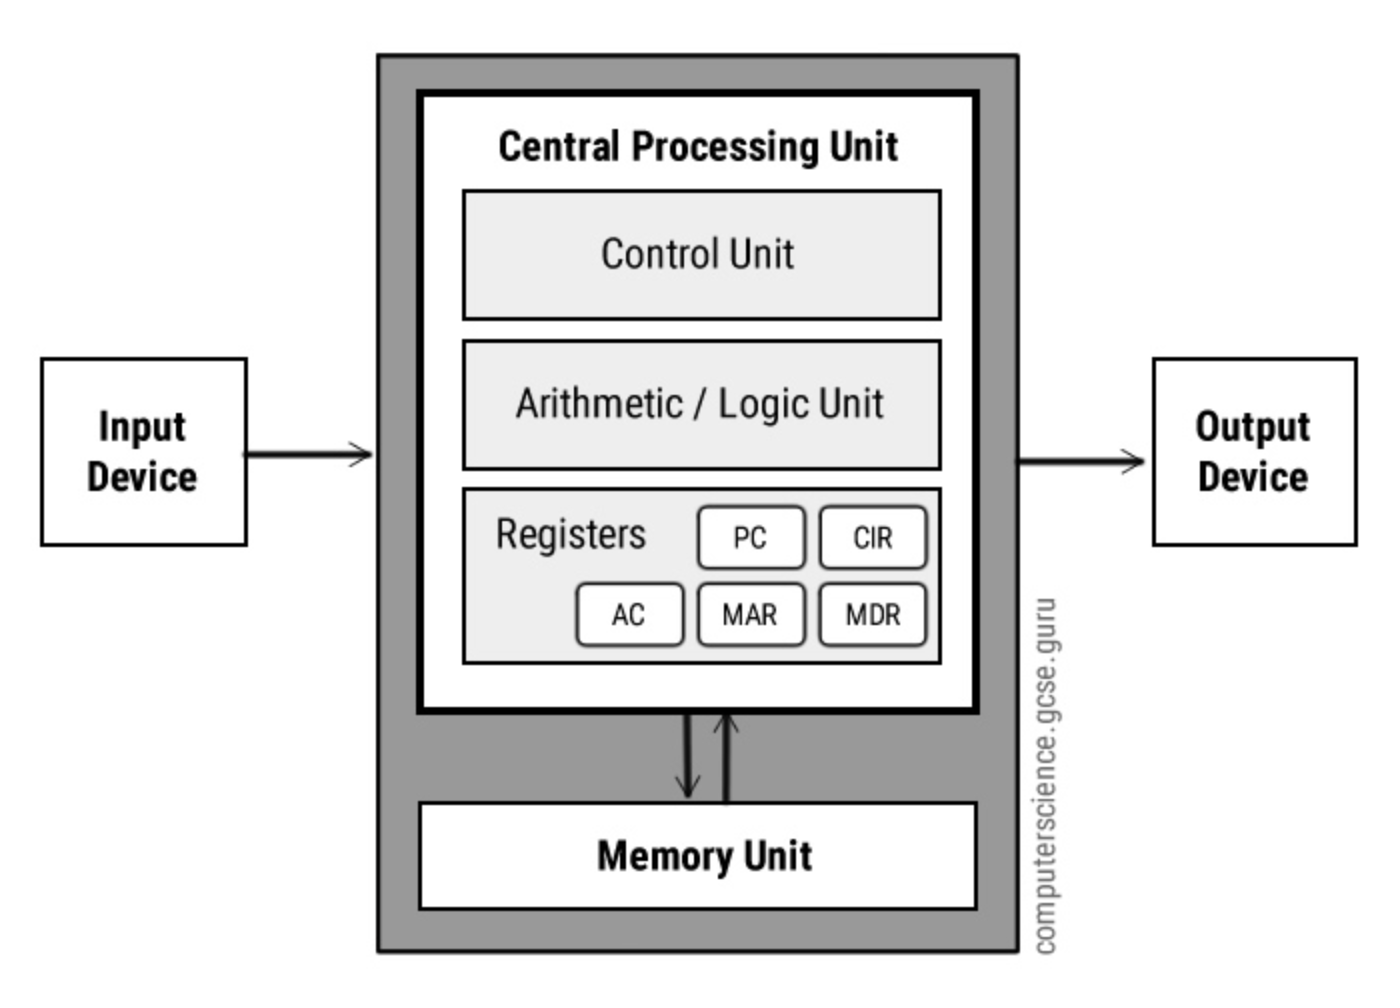
\includegraphics[scale = 0.3]{1.png}}
    \end{center}
            \end{tcolorbox}

            \begin{tcolorbox}[colback=blue!5!white,colframe=blue!50!black,title=2. Ismertesse a determinisztikus véges automata megadását és működését!]
        \begin{itemize}
            \item M automata, input: 0,1-ből álló tetszőleges hosszúságú string. Output: eddig páros számú 0 volt az inputban?
            \item \(M=(S, \Sigma ,T,s,A) ,\hspace{10pt} ahol\)
            \item \(\Sigma ={0,1} \hspace{10pt} input\)
            \item S = {S1,S2}, állapot
            \item s = S1, start
            \item A = {S1}, kimenet (S1-nél igaz)
            \item T állapotátmenet-táblázat
        \end{itemize}
        \begin{center}
            \fbox{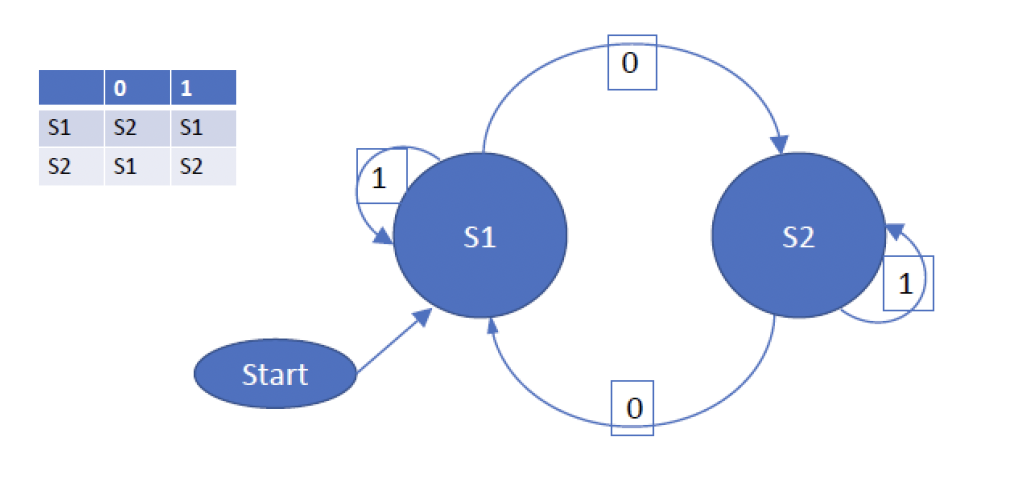
\includegraphics[scale = 0.5]{2.png}}
        \end{center}
            \end{tcolorbox}

            \begin{tcolorbox}[colback=blue!5!white,colframe=blue!50!black,title= 3. Ismertesse a Turing-gép felépítését és működését!]
            \begin{itemize}
                \item Végtelen, cellákra osztott szalag. A cellában lehet szimbólum, vagy üres. Az adatok, a műveletek és eredemények cellái véges számúak, ezentúl a szalag üres.
                \item \textbf{Író/olvasó fej:} egyszerre egy cellával foglalkozik. A cellát írhatja, olvashatja, és törölheti. A szalagon jobbra/balra is lépkedhet, tartalom változás nélkül.
                \item \textbf{Vezérlőegység:} állapotai be vannak számozva, és végesek (véges állapotú automata). A működést helyettesítési táblázat adja meg (állapot+művelet+adat-> új állapot, eredmény, fejmozgás).
                \item \textbf{Matematikailag:} 5-10 elemből álló szabály halmaz
                \item \textbf{Informatikailag:} szalag = memória, vezérlőegység = CPU, fej = busz
                \item CT1-nek megfelelően rekurzióra is alkalmasnak kell lennie: veremtár(stack).
            \end{itemize}
            \begin{center}
                \fbox{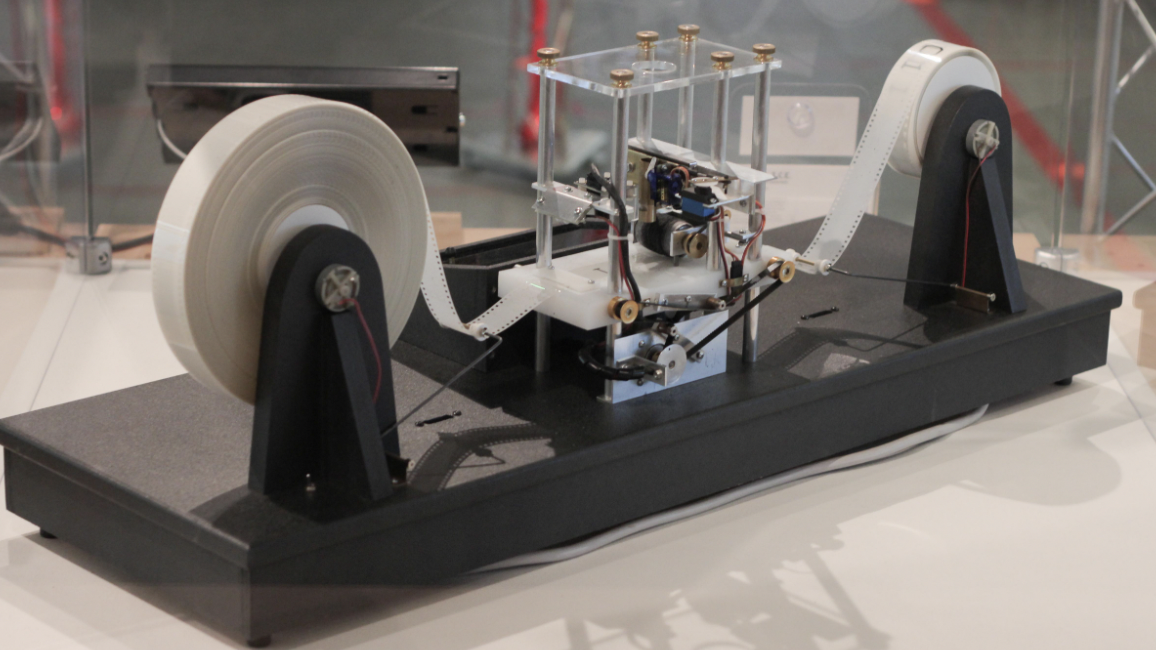
\includegraphics[scale = 0.5]{1_1.png}}
            \end{center}
            \end{tcolorbox}

            \begin{tcolorbox}[colback=blue!5!white,colframe=blue!50!black,title= 4. Ismertesse az algoritmus köznyelvi és matematikai és Turing-géppel megfogalmazott definícióját!]
                \begin{itemize}
                    \item Emberi nyelven megfogalmazott feladat, cselekvéssorozat. (köznyelv)
                    \item Az algoritmusra nem létezik formális matematikai definíció.
                    \item A megoldási eljárást akkor tekintjük algoritmusnak, ha bármilyen bemenet esetén véges számú lépés után eredményt kapunk (a Turing gép megáll).
                \end{itemize}
                \begin{center}
                    \fbox{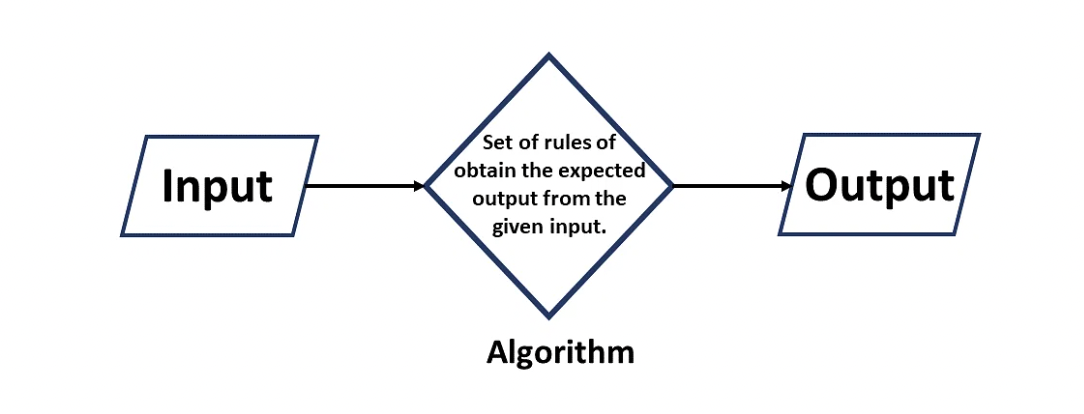
\includegraphics[scale = 0.6]{4.png}}
                \end{center}
            \end{tcolorbox}

            \begin{tcolorbox}[colback=blue!5!white,colframe=blue!50!black,title= 5. Ismertesse az algoritmusok komplexitásának meghatározását! Mondjon példát gyakori komplexitás típusokra!]
                \begin{itemize}
                    \item \textbf{Exponenciális/faktoriális komplexitás:} Az algoritmus futási ideje exponenciálisan növekszik az input méretével. Pl: faktoriális számítás, ahol az algoritmus futási ideje N faktoriálisával arányos, tehát \(O(N!)\)
                    \item \textbf{Polinomiális komplexitás:} Az algoritmus futási ideje polinomiálisan növekszik az input méretével. Példa erre a buborékrendezés algoritmus, ahol az algoritmus futási ideje N négyzetével arányos, tehát \(O(N^2)\)
                    \item \textbf{Lineáris komplexitás:} Az algoritmus futási ideje lineárisan növekszik az input méretével. Példa erre a lineáris keresés algoritmus, ahol az algoritmus futási ideje lineárisan arányos az input méretével, tehát \(O(N)\)
                    \item \textbf{Logaritmikus komplexitás:} Az algoritmus futási ideje logaritmikusan növekszik az input méretével. Példa erre a bináris keresés algoritmus, ahol az algoritmus futási ideje logaritmikusan arányos az input méretével, tehát \(O(log N)\)
                    \item \textbf{Konstans komplexitás:} Az algoritmus futási ideje állandó marad az input méretétől függetlenül. komplexitása: \(O(1)\)
                \end{itemize}
                \begin{center}
                    \fbox{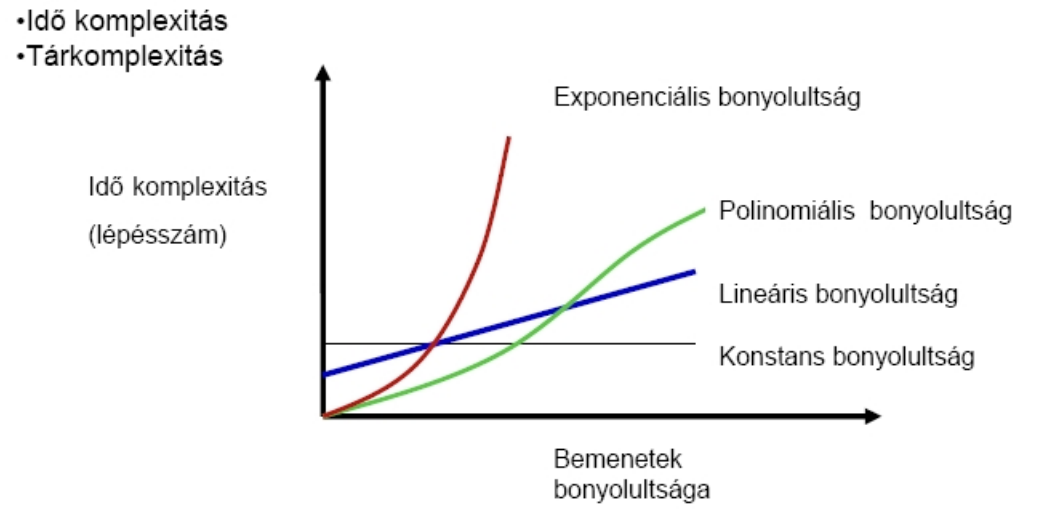
\includegraphics[scale = 0.5]{13.png}}
                \end{center}
            \end{tcolorbox}

            \begin{tcolorbox}[colback=blue!5!white,colframe=blue!50!black,title= 6. Ismertesse a 2 bemenetű logikai függvényeket! Ezek közül néhányat nevezzen is el!]
                \begin{itemize}
                    \item 2 (független) változó esetén:
                    \begin{center}
                        \fbox{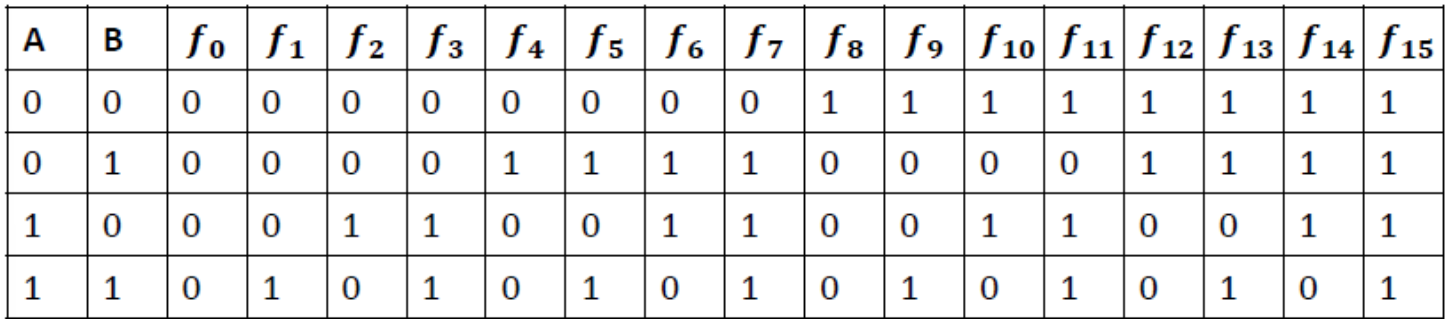
\includegraphics[scale = 0.5]{6_1.png}}
                    \end{center}
                    \(f_1: AND;\hspace{5pt}f_7: OR;\hspace{5pt}f_6: XOR;\hspace{5pt}f_8: NOR;\hspace{5pt}f_{14}: NAND;\hspace{5pt}f_0: 0;\hspace{5pt}f_{15}: 1;\)
                    \item 
                \end{itemize}
                \textbf{Ismertesse (indoklással) az n bemenetű logikai függvények számát!}
                \begin{itemize}
                    \item \(n\) bemenet esetén: \(n\) darab bemenő változó, mindegyiknek 2 értéke van, vagyis
                    \(2n\) bemeneti kombinációhoz 2 elemet rendelünk, azaz: \(2^{2^n} \) darab függvény lesz (2 változó esetén 16 db függvény lesz).
                \end{itemize}
            \end{tcolorbox}

            \begin{tcolorbox}[colback=blue!5!white,colframe=blue!50!black,title= 7. Ismertesse a számítógépes rendszer logikai felépítését!]
                \begin{center}
                    \fbox{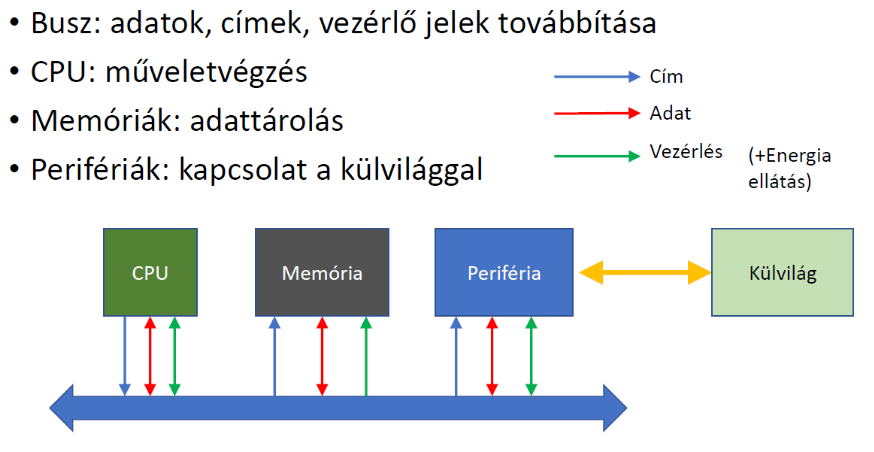
\includegraphics[scale = 0.8]{7_1.png}}
                \end{center}
                \begin{itemize}
                    \item \textbf{Busz:} párhuzamos (manapság soros) jel köteg.
                    \item \textbf{Busz szélességek:} egyszerre átvihető adat mérete.
                    \item \textbf{Adatbusz:} 8 bit (C64, ZX spectrum), 16 bit (IBM PC, pic24), 32 bit (IBM 386-486-Pentium) , 64 bit PC manapság. Szinte mindig az akkumulátor regiszermérete.
                    \item \textbf{Címbusz:} memória maxméretét adja meg. 8 bites CPU-nál gyakran 16 bites (65536 cella), IBM PC-nél 20 bites, i9: 128 GB címezhető meg.
                    \item Ha a memória-vezérlő is a CPU része, a címbusz csak belül jelenik meg.
                \end{itemize}
            \end{tcolorbox}

            \begin{tcolorbox}[colback=blue!5!white,colframe=blue!50!black,title= 8. Ismertesse az 1 bites teljes összeadó példáján keresztül a kombinációs logikai hálózatok elvét!]
                \textbf{1 bites teljes összeadó igazságtáblája:}
                \begin{center}
                    \fbox{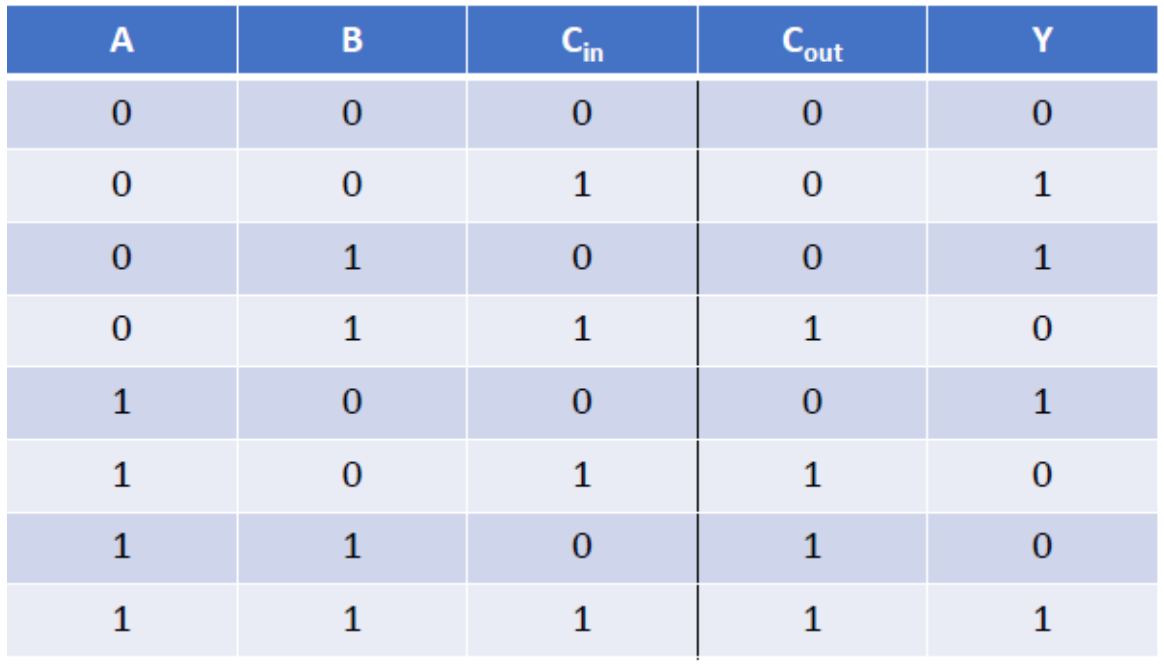
\includegraphics[scale = 0.5]{8_1.png}}
                \end{center}
                \begin{itemize}
                    \item \textbf{Bemenetek:} \(A,\hspace{3pt}B,\hspace{3pt}C_{in}\); \textbf{Kimenetek:} \(Y,\hspace{3pt}C_{out}\)
                    \item \(Y\hspace{3pt}=\hspace{3pt}A\hspace{3pt}xor\hspace{3pt}B\hspace{3pt}xor\hspace{3pt}C\)
                    \item \(C_{out} = (A\hspace{3pt}and\hspace{3pt}B)\hspace{3pt}or\hspace{3pt}(A\hspace{3pt}and\hspace{3pt}C_{in})\hspace{3pt}or\hspace{3pt}(B\hspace{3pt}and\hspace{3pt}C_{in})\)
                    \item A kombinációs logikai hálózatok kimenetei csak a bementektől függnek. Minden kimenetet egy függvény ír le.\((F_1(X_1, X_2, ... X_n))\)
                \end{itemize}
            \end{tcolorbox}

            \begin{tcolorbox}[colback=blue!5!white,colframe=blue!50!black,title= 9. Ismertesse számpéldán keresztül a negatív egész számok kettes komplemens ábrázolását!]
                \begin{itemize}
                    \item \textbf{Signed (előjeles):} számoknál a legfelső bit értéke egy, ha a szám negatív. Ezzel a tartományt lefeleztük, de negatívba is mehetünk.
                    \item \textbf{Unsigned:} nincs előjelbit, csak pozitív számok
                \end{itemize}
                \begin{center}
                    \fbox{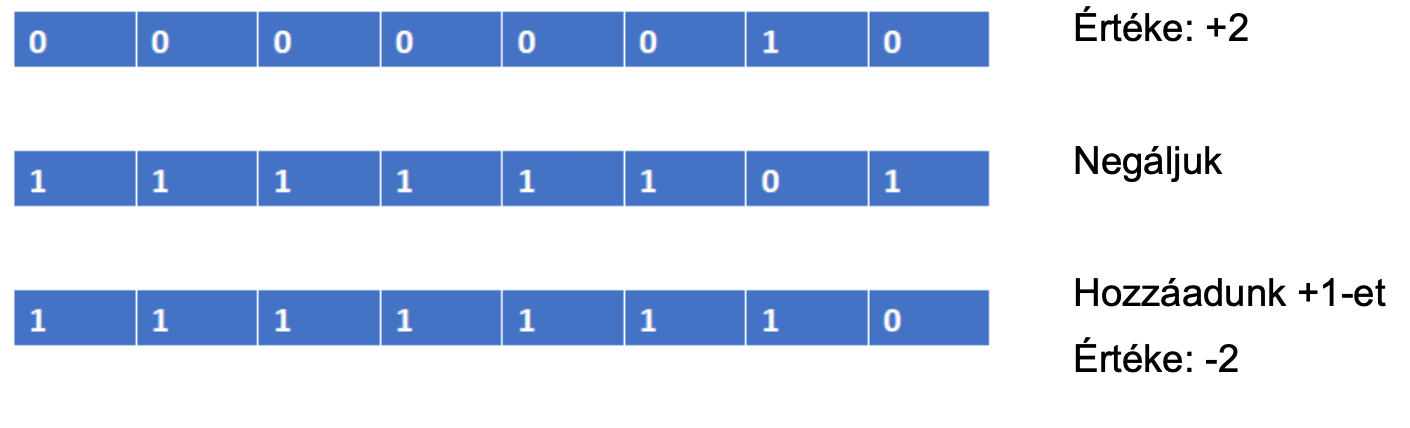
\includegraphics[scale = 0.5]{9_1.png}}
                \end{center}
            \end{tcolorbox}

            \begin{tcolorbox}[colback=blue!5!white,colframe=blue!50!black,title= 10. Ismertesse az S-R tároló példáján keresztül a szekvenciális logikai hálózatok elvét!]
                \begin{itemize}
                    \item A szekvenciális hálózat a bemenetektől és a hálózat belső állapotától (amelyet a bemeneti jelek is okoztak) is függ.
                    \begin{itemize}
                        \item \textbf{Aszinkron:} nincs ütemező órajel
                        \item \textbf{Szinkron:} csak órajelnél vált állapotot (pl: cpu)
                    \end{itemize}
                \end{itemize}
                \begin{center}
                    \fbox{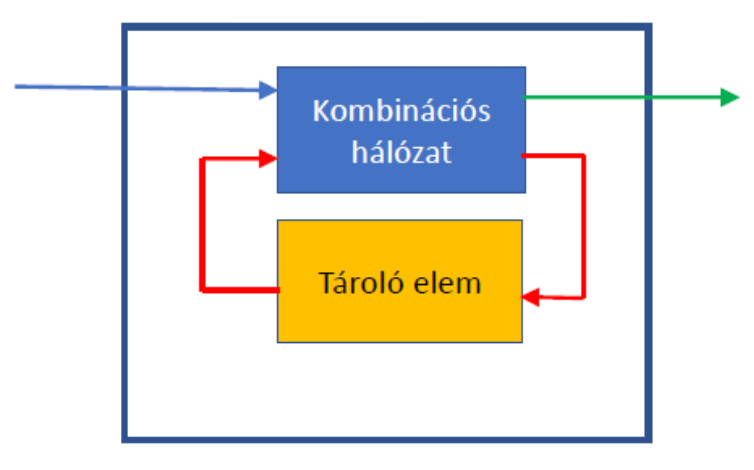
\includegraphics[scale = 0.5]{10_1.png}}
                \end{center}
                    \begin{itemize}
                        \item \textbf{S-R tároló:}
                        \begin{itemize}
                        \item S: “set” 1-re állítja a kimenetet
                        \item R: “reset” 0-ra állítja a kimenetet
                        \item S = 0 és R = 0 esetén tartja az előző értéket (memória)
                        \item S = 1 és R = 1 esetén érvénytelen állapot, mert Q és Q is 0 lenne.
                        \end{itemize}
                    \end{itemize}
                    \begin{center}
                        \fbox{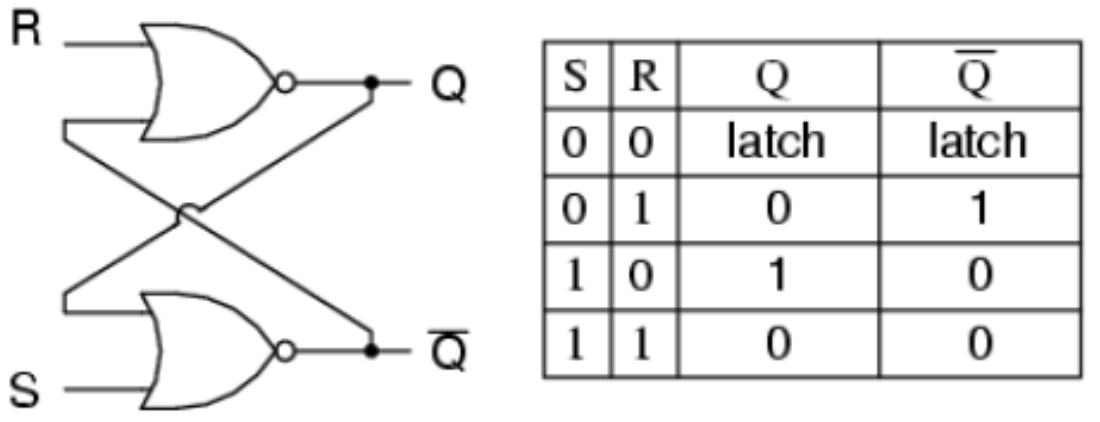
\includegraphics[scale = 0.5]{10_2.png}}
                    \end{center}
            \end{tcolorbox}

            \begin{tcolorbox}[colback=blue!5!white,colframe=blue!50!black,title= 11. Ismertesse a D tároló felépítését és működését!]
                \begin{itemize}
                    \item \textbf{Működése:}
                    \begin{itemize}
                        \item A D tárolóba érkező adat (D) bejut a tároló belső áramköreibe, és várakozik az órajel (CLK) jelre.
                        \item Amikor az órajel jele pozitív, a tároló belső áramkörei elvégzik a szükséges műveleteket.
                        \item Az adat (D) a CLK jel hatására frissül, és bekerül a tárolóba.
                        \item A tárolt adat azonnal megjelenik a kimeneten (Q), és ezt a kimenetet a következő CLK jelre változhat.
                    \end{itemize}
                \end{itemize}
                \begin{center}
                    \fbox{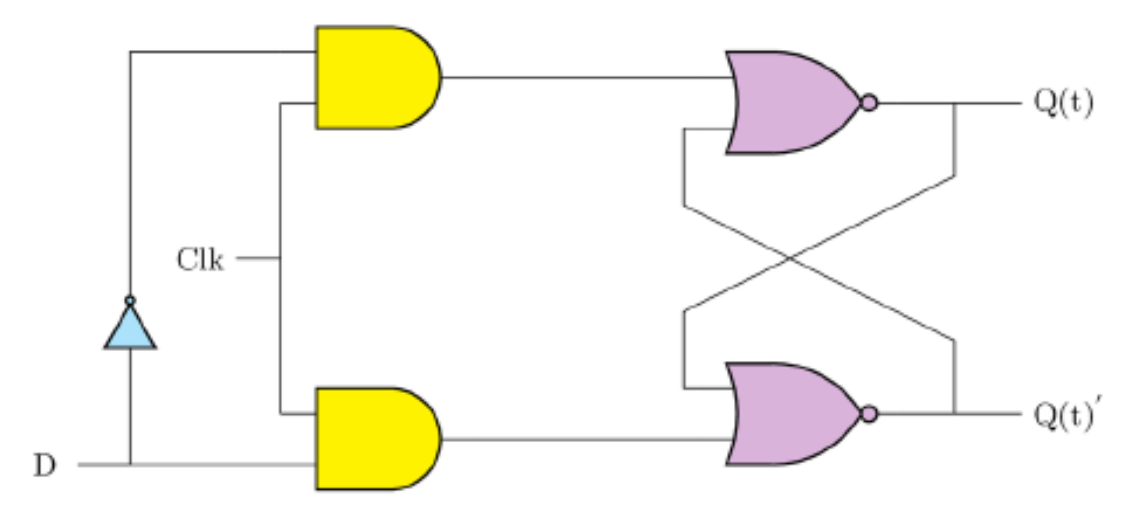
\includegraphics[scale = 0.5]{11_1.png}}
                \end{center}
                \textbf{Melyik tároló tartalmaz a számítógépben D tárolót?}
                \begin{itemize}
                    \item RAM, SSD, HDD
                \end{itemize}
            \end{tcolorbox}
            
            \begin{tcolorbox}[colback=blue!5!white,colframe=blue!50!black,title= 12. Ismertesse a tárolók hierarchia szintjeit!]
                \begin{itemize}
                    \item \textbf{Regiszterek:} A regiszterek a CPU belső tárolói, amelyek nagyon gyors hozzáférést biztosítanak az adatokhoz. A regiszterek közvetlenül a CPU-ban találhatóak, és az utasítások végrehajtásához és az adatok köztes tárolásához használhatóak.
                    \item \textbf{Cache:} A cache olyan kis méretű, gyors és közel a processzorhoz elhelyezkedő tároló, amely az aktuálisan leggyakrabban használt adatokat és utasításokat tárolja. Célja, hogy csökkentse a memória-hozzáférési időt és javítsa a rendszer teljesítményét.
                    \item \textbf{Operatív tár (RAM):} Az operatív tár az adatok és utasítások átmeneti tárolására szolgál a számítógépben. Ez a tár rendelkezik nagyobb kapacitással, mint a regiszterek vagy a cache, de lassabb hozzáférést biztosít. Az adatok ideiglenesen tárolódnak itt a futó programok számára.
                    \item \textbf{Mágneses/SSD direkt elérésű háttértár:} Ez a tároló típus olyan háttértár, amely mágneses lemezeket (merevlemezeket) vagy szilárdtest meghajtókat (SSD) használ. Ezek a tárolók nagyobb kapacitással rendelkeznek, mint az operatív tár, és lehetővé teszik az adatok hosszú távú tárolását.
                    \item \textbf{Szekvenciális elérésű háttértár:} Ez a tároló típus olyan adathordozókat használ, mint például a szalagok. A szekvenciális tárolóknál az adatok egymás után találhatók, és az adatokhoz való hozzáférés sorrendben történik. A szekvenciális elérés lassabb, mivel az adatokat folyamatosan kell olvasni vagy írni a szalag vagy más hordozó mentén.
                \end{itemize}
            \end{tcolorbox}
            
            \begin{tcolorbox}[colback=blue!5!white,colframe=blue!50!black,title= 13. Ismertesse a CPU részeit és működését egy utasítás végrehajtási folyamatában!]
            A CPU (Central Processing Unit - központi feldolgozó egység) a memóriából olvassa a
            végrehajtás alatt lévő program bináris utasításait. Az utasításkészlete fontos jellemzője.
            A mikroprocesszor egy chipen kialakított áramkör, mely a számítógép CPU-jának a
            funkcióját látja el. Végrehajtandó utasítás memória címe programszámláló regiszterben. Utasítás beolvasás (fetch) memóriából.
            Utasítás dekódolás, ha további paraméterek is vannak a memóriában,
            beolvasásra kerülnek.
            Utasítás végrehajtása, eredmény (ha van) tárolása.
            Következő utasítás címének megadása (programszámláló regiszter a
            végrehajtott utasítás hosszával inkrementálódik).\\
            \\
            \textbf{Részei:}  
                \begin{itemize}
                    \item \textbf{ALU}
                    \begin{itemize}
                        \item Aritmetikai és logikai műveletek végzése
                        \item Összeadás, kivonás, fixpontos szorzás, osztás (léptetések), lebegőpontos aritmetikai
                    műveletek (korábban koprocesszor), egyszerű logikai műveletek.
                    \end{itemize}
                    \item \textbf{Utasítás dekódoló és vezérlő egység}
                    \begin{itemize}
                        \item Felismeri, elemzi (dekódolja) a gépi nyelvű program utasításait, az utasítások alapján működtetik a CPU többi segítségét 
                    \end{itemize}
                    \item \textbf{Regiszterek}
                    \begin{itemize}
                        \item Chipen belüli, közvetlen elérésű tároló elemek.
                        \item Feladatuk műveletvégzéskor az operandusok tárolása, illetve a címek előállítása.
                    \end{itemize}
                \end{itemize}
                \begin{center}
                    \fbox{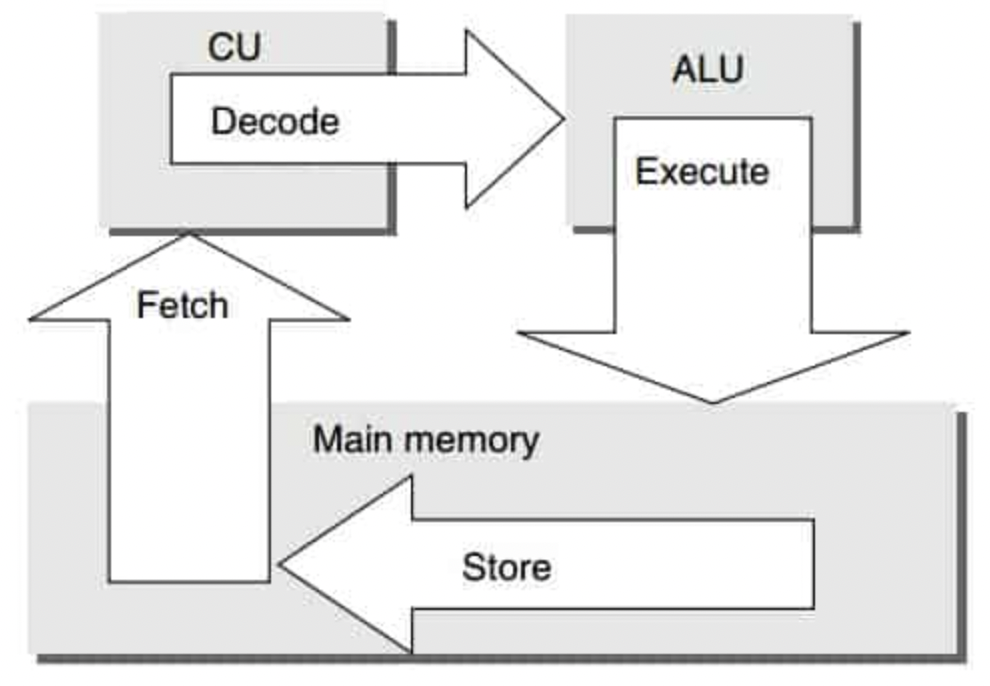
\includegraphics[scale = 0.7]{13_2.png}}
                \end{center}
            \end{tcolorbox}
            
            \begin{tcolorbox}[colback=blue!5!white,colframe=blue!50!black,title= 14. Ismertesse a periféria csatolási módszereket{,} módszerenként kitérve az adott módszer előnyére{,} és hátrányára! Part 1.]
                \begin{itemize}
                    \item \textbf{Polling}
                    \begin{itemize}
                        \item A periféria állapotát le kell kezelni: pl. észre kell venni, ha leütöttek egy billentyűt.
                        \item Ennek legegyszerűbb módja az ún. pollozás/polling: a program bizonyos időközönként kiolvassa a perifériát, ha nincs változás, foglalkozik a többi programmal, ha változás van, lekezeli a változást, majd foglalkozik a többi programmal.
                        \item A periféria változása a főprogramhoz képest aszinkron bekövetkezésű (vagyis nem tudjuk, hogy mikor kell beavatkozni).
                        \item A módszer nem hatékony: túl sok utasítás megy el felesleges lekérdezéssel, a főprogramból gyakran kell lekérdezést kérdezni,
                    \end{itemize}
                    \item \textbf{IRQ}
                    \begin{enumerate}
                        \item Egészítsükki a perifériát egy plusz kimeneti lábbal: ezen küldjön aktív értéket, ha állapotváltozás miatt „figyelemre” van szüksége.
                        \item Ezt a lábat nevezzük el „interruptrequest”/megszakítás kérő lábnak.
                        \item A lábat kössük be a CPU-ba! (a gyakorlati megvalósítás bonyolultabb: pl. azonosítani kell, hogy melyik
                        periféria volt a megszakítás kérő).
                        \item A megszakítási kérelemre a CPU futtasson le egy IRQ kezelő függvényt. A függvény címe a memóriában fix helyen, IVT-ben van tárolva. A függvényt úgy kell megírni, hogy ne rontsa el a regiszterek értékét, mert az IRQ bármikor jöhet.
                    \end{enumerate}
                    \textbf{Felhasználás:}
                    \begin{itemize}
                        \item Hardver hibák (memória hiba, busz hiba) lekezelése
                        \item Szoftver hibák (0-val osztás, védett memóriaterületre hivatkozás, verem alul/felülcsordulás) lekezelése
                        \item Idő kezelése (1s-onként irqaktualizálja a rendszeridőt)
                        \item Szoftveresen is hívható, intel-nél utasítás van rá: operációs rendszer belépési pontjai.
                        \item Maszkolhatómegszakítás: utasítással letiltható, ekkor nem fut le az irqszubrutin
                        \item Nem maszkolhatómegszakítás (NMI) szoftverből nem tiltható le.
                        \item A megszakítások prioritási sorba állíthatók: a nagyobb prioritású irqmegszakíthatja a kisebb prioritású irqkiszolgálását, fordítva nem.
                    \end{itemize}
                \end{itemize}
            \end{tcolorbox}

            \begin{tcolorbox}[colback=blue!5!white,colframe=blue!50!black,title= 14. Ismertesse a periféria csatolási módszereket{,} módszerenként kitérve az adott módszer előnyére{,} és hátrányára! Part 2.]
                \begin{itemize}
                    \item \textbf{DMA nélkül}
                    \begin{itemize}
                        \item  Nagymennyiségű adat átvitele a háttértárról (periféria)
                        \item CPU megcímzi a perifériát (megadja, hogy hol található az adat) a buszon keresztül
                        \item Periféria szolgáltatja az adatot (idő!) Az adat a CPU regiszterébe kerül (buszon keresztül)
                        \item A CPU a memóriába teszi az adatot a regiszterből.
                        \item Következő bájt a memória következő címére a háttértárról
                        \item CPU mással nem tud közben foglalkozni.
                    \end{itemize}
                    \begin{center}
                        \fbox{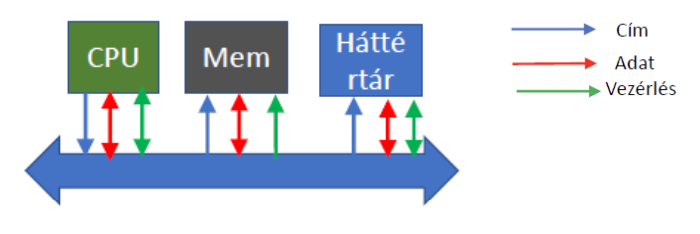
\includegraphics[scale = 0.7]{14_2_1.png}}
                    \end{center}
                    \item \textbf{DMA}
                    \begin{itemize}
                        \item A művelet közben nincs nagy számítás igény: buszt kell vezérelni, címet növelni 1-gyel.
                        \item Erre a műveletre készülhet egy speciális áramkör: DMA vezérlő.
                    \end{itemize}
                    \begin{enumerate}
                        \item A CPU megmondja a DMA vezérlőnek, hogy honnan, hova, hány bájtot.
                        \item A DMA vezérlő elkéri a buszt a CPU-tól, ha annak éppen nincs rá szüksége (plbelső művelet zajlik). A CPU lekapcsolja a buszmeghajtókat.
                        \item A DMA vezérlő átvisz 1 bájtot a perifériából, a saját adatregiszerébe(olvasás esetén).
                        \item A DMA vezérlő által elkért buszon átvisz 1 bájtot a memóriába. Írás esetén a két lépés fordított sorrendben.
                        \item A DMA vezérlő visszaadja a buszt
                        \item DMA vezérlő újra elkéri a buszt.
                        \item Az utolsó bájt átvitele után nem kéri el a buszt, egy IRQ-n keresztül jelzi, hogy az átvitel kész.
                        \item A busz elkérés neve: busz arbritráció.
                        \item Dinamikus memória frissítésére is kiváló!
                    \end{enumerate}
                \end{itemize}
                \begin{center}
                    \fbox{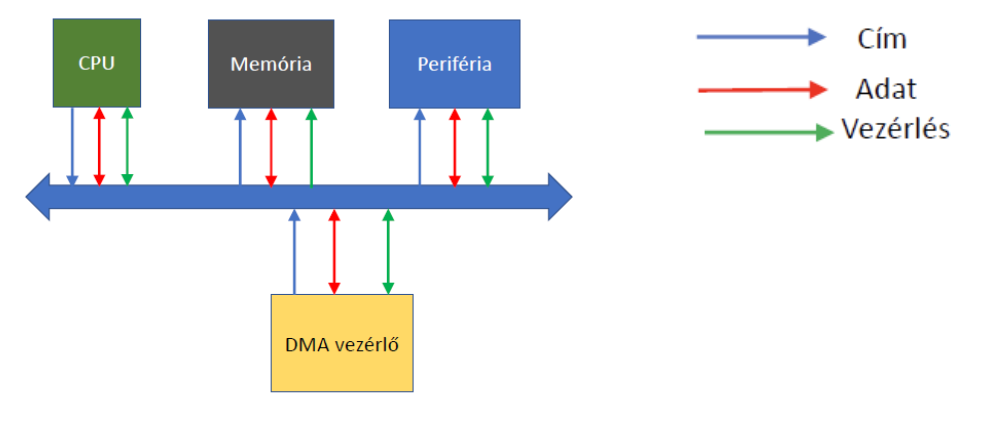
\includegraphics[scale = 0.6]{14_2_2.png}}
                \end{center}
            \end{tcolorbox}
            
            \begin{tcolorbox}[colback=blue!5!white,colframe=blue!50!black,title= 15. Ismertesse az alapvető algoritmus-elemeket a Böhm-Jacopini tétel alapján!]
                \begin{itemize}
                    \item \textbf{Böhm-Jacopini tétele:} Minden algoritmus leírható 3 logikai struktúrával:
                    \item \textbf{Rákövetkezés (konkatenáció):}
                    \begin{itemize}
                        \item Az utasítások egymás után hajtódnak végre
                        \item Külön kulcsszó nem tartozik hozzá (alapesetben is egymás után hajtjuk végre az utasítások, a címek szerint növekvő sorrendben.) 
                        \item C-ben az egymás alá írt utasítások egymás utáni címekre kerülnek.
                    \end{itemize}
                    \begin{center}
                        \fbox{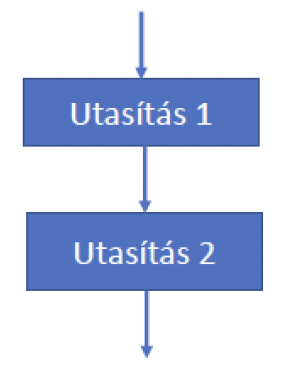
\includegraphics[scale = 0.5]{16_1.png}}                            
                    \end{center}
                    \item \textbf{Választás (alternáció):}
                    \begin{itemize}
                        \item Egy logikai feltétel függvényében kerül végrehajtásra az utasítás
                        \item Feltétel hamis értéke esetén is megadható másik utasítás 
                        \item C-ben: \(if (condition)\hspace{8pt} command_{true} ;\hspace{8pt} command_{false};\)
                    \end{itemize}
                    \begin{center}
                        \fbox{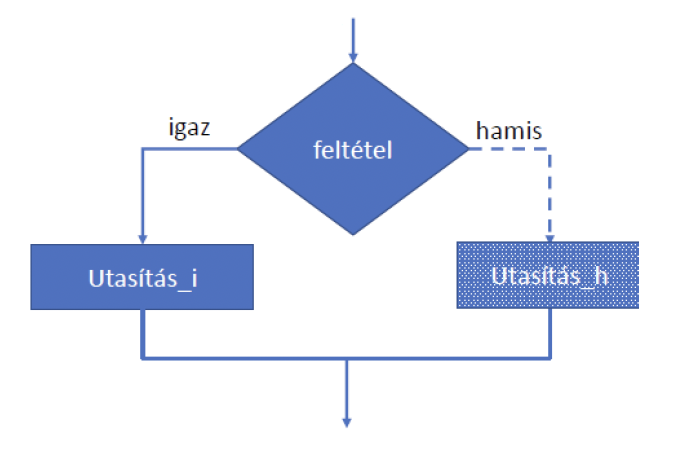
\includegraphics[scale = 0.5]{16_2.png}}
                    \end{center}
                    \item \textbf{Ciklus (iteráció):}
                    \begin{itemize}
                        \item Egy feltételtől függően ismételjük az utasításokat
                        \item A feltétel és az utasítás egymáshoz képesti elhelyezkedése miatt előltesztelt és hátúltesztelt
                    \end{itemize}
                \end{itemize}
                \begin{center}
                    \fbox{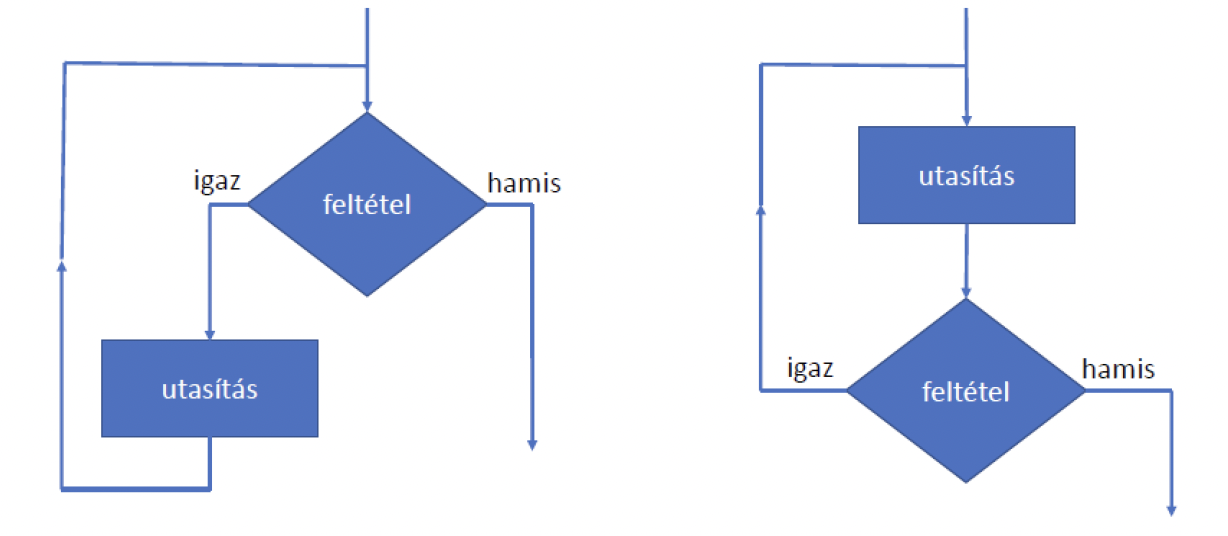
\includegraphics[scale = 0.5]{16_3.png}}
                \end{center}
            \end{tcolorbox}
            
            \begin{tcolorbox}[colback=blue!5!white,colframe=blue!50!black,title= 16. Ismertesse az alapvető adatszerkezet típusokat és ezek műveleteit!]
                \begin{itemize}
                    \item \textbf{Adatszerkezet:} egyszerű vagy összetett alapadatok rendszerének matematikai, logikai modellje
                    \item \textbf{Típusok:}
                    \begin{itemize}
                        \item \textbf{Tömb (Array):} (lineáris, egy vagy több dimenziós)
                        \item \textbf{Rekord (Record):} összetartozó adatok egy példányhoz
                        \item \textbf{Kapcsolt lista (Linked list):} a kapcsolati információt is tároljuk
                        \item \textbf{Gráf (Tries):} két kapcsolódó adathalmaz: csomópontok és élek
                        \item \textbf{Fa (Trees):} Hurok nélküli gráf. Általános és bináris fa
                        \item \textbf{Verem (Stacks):} LIFO (Last In First Out)
                        \item \textbf{Sor (Queue):} FIFO (First In First Out)
                    \end{itemize}
                    \item \textbf{Műveletek}
                    \begin{itemize}
                        \item \textbf{Bejárás:} az elemek elérése.
                        \item \textbf{Keresés:} adott feltételnek megfelelő elemek kiválasztása.
                        \item \textbf{Beszúrás:} új adat beillesztése az adatszerkezetbe
                        \item \textbf{Törlés:} adat eltávolítása az adatszerkezetből
                        \item \textbf{Rendezés:} adatok logikai sorrendbe állítása
                        \item \textbf{Összeválogatás:} különböző rendezett elemhalmazotból új elemhalmaz kialakítása.
                    \end{itemize}
                \end{itemize}
                \begin{center}
                    \fbox{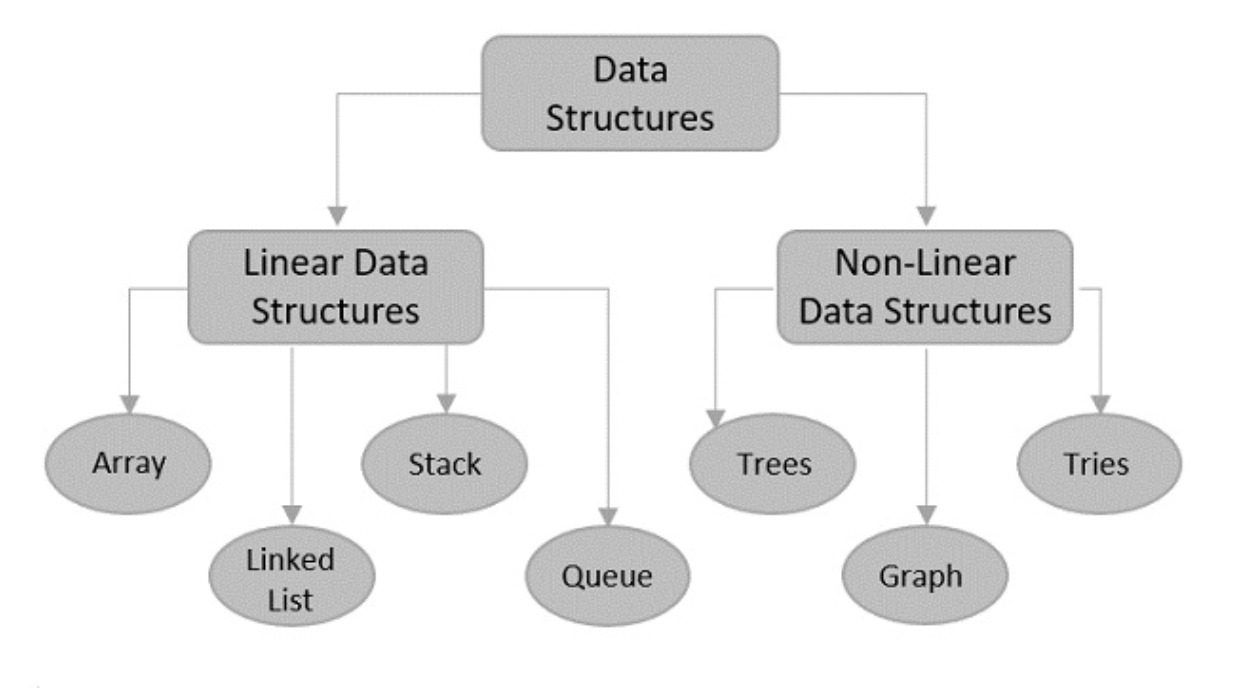
\includegraphics[scale = 0.5]{16_4.png}}
                \end{center}
            \end{tcolorbox}
            
            \begin{tcolorbox}[colback=blue!5!white,colframe=blue!50!black,title= 17. Ismertesse a lineáris és a többdimenziós tömbök memóriamodelljét!]
                \textbf{Lineáris tömbök:}
                \begin{itemize}
                    \item Azonos típusú (méretű) adatelemek
                    \item Az elemekre indexsegítségével hivatkozunk
                    \item Egymást követő memóriacímeken tároljuk, folytonosterületen
                    \item Egy elemhez bejárás nélkül férünk hozzá, konstans idővel
                    \item Beszúrás/törlés nem hatékony!
                    \item i-edik elem memória címe = tömb első elemének címe+i*adatmérete. A pointer az adat méretét tudja! Ezért *(t+i)
                \end{itemize}
                \begin{center}
                    \fbox{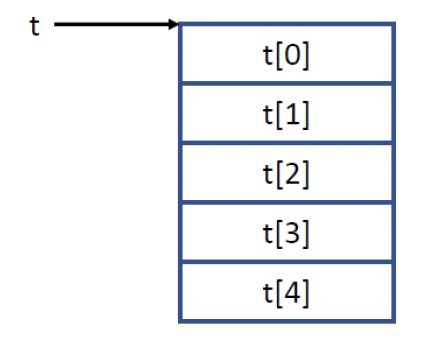
\includegraphics[scale = 0.5]{18_1.png}}
                \end{center}
                \textbf{Többdimenziós tömbök:}
                \begin{itemize}
                    \item A memória lineáris. Több dimenziós tömböt kétféleképpen tárolhatunk:
                    \item A tömb elemei pointerek, amelyek tömbök (C és C++). Duplaindirekció: int **t; hivatkozás: \(t[i][j]\)
                    \item A programozó vagy a fordító leképezi az idexeket a lineáris memóriába. Pl. \(C\sharp \hspace{5pt}t[i,j]\)
                    \item \([i,j]\)-edik elem címe egy m*n-estömbben: tömb kezdőcíme + (n*i+j)*adatmérete
                \end{itemize}
                \begin{center}
                    \fbox{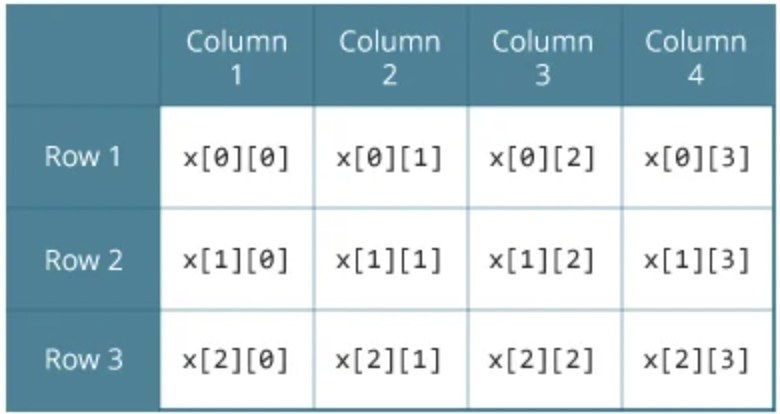
\includegraphics[scale = 0.8]{18_2.png}}
                \end{center}
            \end{tcolorbox}
            
            \begin{tcolorbox}[colback=blue!5!white,colframe=blue!50!black,title= 18. Ismertesse a kapcsolt lista adatszerkezet felépítését és gyakori műveleteit!]
                \textbf{A kapcsolt lista adatszerkezet felépítése:}
                \begin{itemize}
                    \item Csomópontokból áll, amelyek tartalmazzák az adatot és egy mutatót a következő csomópontra.
                    \item Az utolsó csomópont mutatója NULL, jelezve a lista végét.
                \end{itemize}
                \textbf{Gyakori műveletek a kapcsolt listán:}
                \begin{itemize}
                    \item Elem hozzáadása a lista elejéhez (prepend).
                    \item Elem hozzáadása a lista végéhez (append).
                    \item Elem beszúrása adott helyre.
                    \begin{center}
                        \fbox{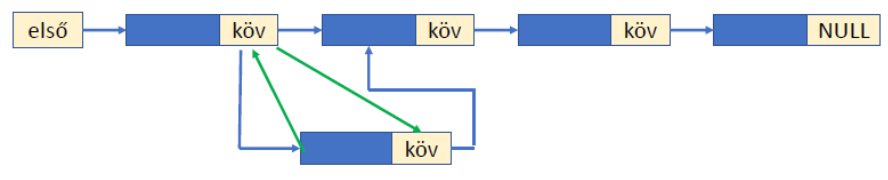
\includegraphics[scale = 0.7]{19_2.png}}
                    \end{center}
                    \item Elem törlése a listából.
                    \begin{center}
                        \fbox{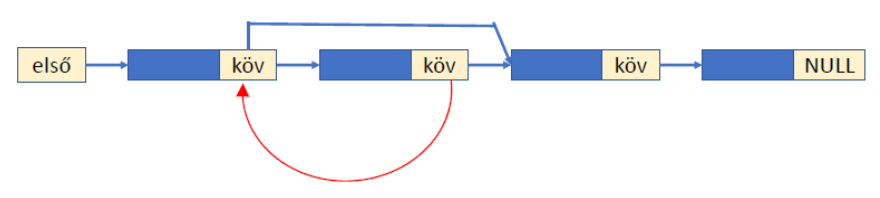
\includegraphics[scale = 0.7]{19_1.png}}
                    \end{center}
                    \item Adott elem keresése a listában.
                    \item Lista méretének lekérdezése.
                    \item Lista kiíratása.
                \end{itemize}
                \textbf{Előnyök:}
                \begin{itemize}
                    \item Dinamikus méret, könnyű bővítés és csökkentés.
                    \item Hatékony beszúrás és törlés az adott helyen.
                    \item Memóriatakarékos, mert csak az aktuális elemekhez szükséges memóriát foglalja le.
                \end{itemize}
                \textbf{Hátrányok:}
                \begin{itemize}
                    \item Random hozzáférés lassú, mert a kereséshez végig kell menni a listán.
                    \item Több memóriaterületet igényel, mert minden csomóponthoz szükséges egy mutató.
                    \item Összekapcsoltság elvesztése, ha valamelyik mutató hibás lesz.
                \end{itemize}
            \end{tcolorbox}
            
            \begin{tcolorbox}[colback=blue!5!white,colframe=blue!50!black,title= 19. Ismertesse a gráf definícióját valamint az alábbi gráfelméleti fogalmakat: út{,} kör{,} összefüggő{,} teljes{,} címkézett{,} súlyozott és irányított!]
                \begin{itemize}
                    \item \textbf{Gráf definíciója:} A gráf egy matematikai struktúra, amely csomópontokból (vagy csúcsokból) és azokat összekötő élekből áll. A gráfot grafikusan ábrázoljuk, ahol a csomópontokat pontokkal, az éleket pedig vonalakkal jelöljük.
                    \item \textbf{Út:} Az út olyan sorozat vagy láncolat, amelyben egymás után következnek a gráf csomópontjai úgy, hogy az élek az egymást követő csomópontokat összekötik.
                    \item \textbf{Kör:} A kör egy olyan út, amely a kezdőpontjába visszatér, vagyis a kör kezdő- és végpontja azonos csomópont.
                    \item \textbf{Összefüggő:} Egy gráf akkor összefüggő, ha bármely két csomópontja között van legalább egy út.
                    \item \textbf{Teljes:} Egy gráf teljes, ha minden csomópontja között van él, azaz bármely két csomópont között van egy-egy él.
                    \item \textbf{Címkézett:} Egy címkézett gráfban a csomópontokhoz vagy élekhez hozzárendelhetünk címkéket vagy jellemzőket, amelyek információt hordoznak a gráf elemeiről.
                    \item \textbf{Súlyozott:} Egy súlyozott gráfban az élekhez hozzárendelünk súlyokat vagy értékeket, amelyek jelzik az élek közötti kapcsolat erősségét vagy távolságát.
                    \item \textbf{Irányított:} Egy irányított gráfban az élek egyirányúak, tehát a csomópontok közötti kapcsolatok egyirányúak lehetnek.
                \end{itemize}
            \end{tcolorbox}
            
            \begin{tcolorbox}[colback=blue!5!white,colframe=blue!50!black,title= 20. Ismertesse a gráfok szomszédsági mátrixát!]
                \begin{itemize}
                    \item \textbf{Szomszédossági mátrix:} \(a_{ij} = 1\), ha \(i\)-ből \(j\)-be halad él, egyébként \(a_{ij}\) = 0
                    \begin{center}
                        \fbox{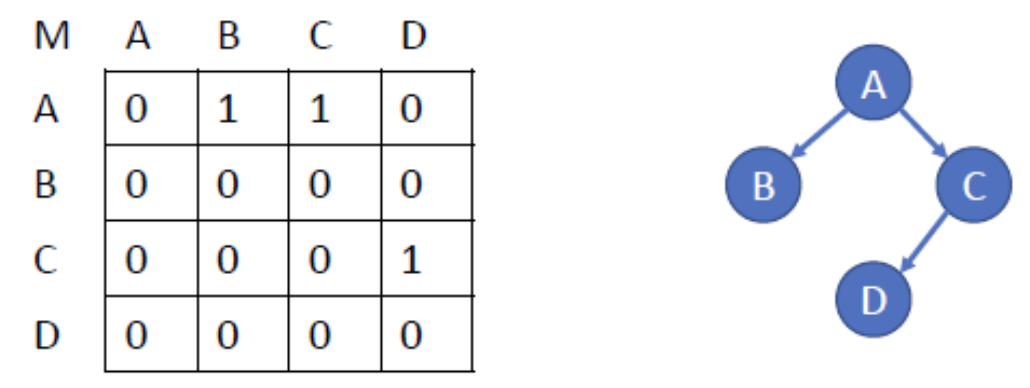
\includegraphics[scale = 0.5]{20_1.png}}
                    \end{center}
                    \item Ha \(M\) a \(G\) gráf szomszédsági mátrixa, akkor \(M^k_{ij}\) -edik eleme az \(i\)-ből a \(j\)-be vezető \(k\) hosszú utak számát adja
                    \begin{center}
                        \fbox{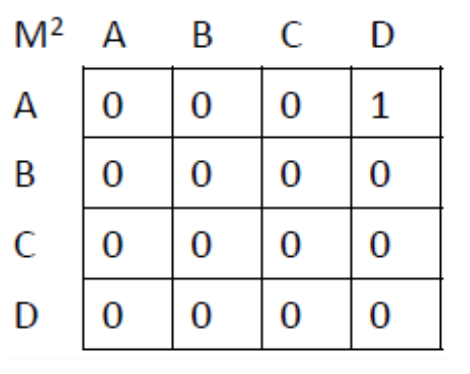
\includegraphics[scale = 0.5]{20_2.png}}
                    \end{center}
                \end{itemize}
            \end{tcolorbox}
            
            \begin{tcolorbox}[colback=blue!5!white,colframe=blue!50!black,title= 21. Ismertesse az általános fa felépítését és tárolását számítógépen!]
                \begin{itemize}
                    \item Elemek véges halmaza (T), amely 
                    \begin{itemize}
                        \item Tartalmaz egy kitüntetett R gyökérelemet
                        \item A többi elem nem nulla diszjunkt részfája T-nek
                    \end{itemize} 
                \end{itemize} 
                \begin{center}
                    \fbox{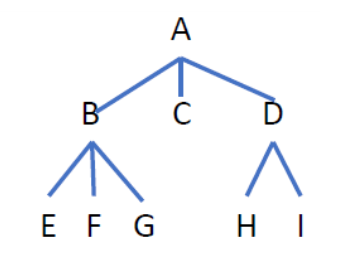
\includegraphics[scale = 0.6]{22_1.png}}
                \end{center}
                \begin{itemize}
                    \item Tárolás 
                    \begin{itemize}
                        \item Info(k) - az elem adatai 
                        \item Gyermek(ek) - az első gyerek index
                        \item Testvér - az első testvér indexe 
                    \end{itemize}
                \end{itemize}
                \begin{center}
                    \fbox{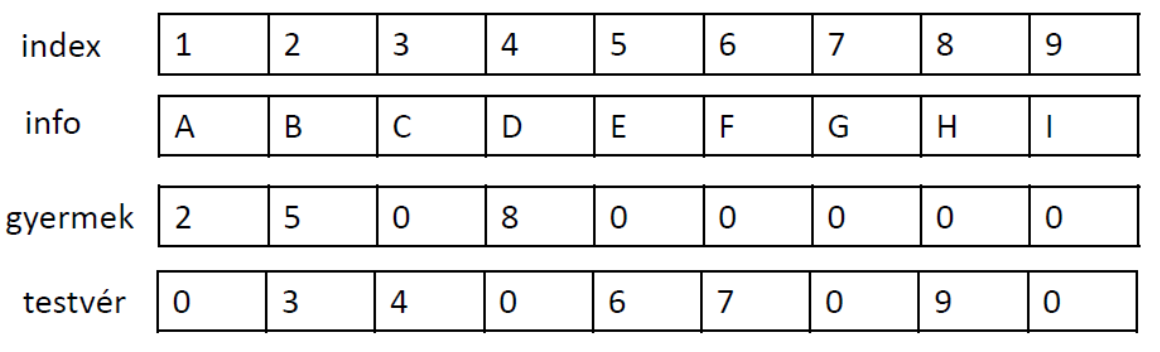
\includegraphics[scale = 0.6]{22_2.png}}
                \end{center}
            \end{tcolorbox}
            
            \begin{tcolorbox}[colback=blue!5!white,colframe=blue!50!black,title= 22. Ismertesse a bináris fák szerkezetét és tárolási lehetőségeit számítógépen!]
                \begin{itemize}
                    \item Elemek véges halmaza, amely, vagy üres, vagy egyetlen T elemhez (gyökér) kapcsolt két diszjunkt T1 és T2 részfa alkotja\\
                    \begin{center}
                        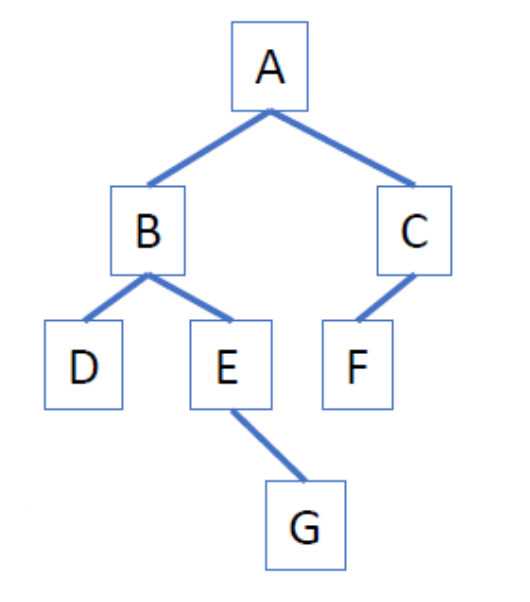
\includegraphics[scale = 0.3]{23_1.png}
                    \end{center}
                    \item \textbf{Gyökérelem:} A
                    \item \textbf{Baloldali részfa:} L(A)=(B,D,E,G)
                    \item \textbf{Jobboldalirészfa:} R(A)=(C,F)
                    \item \textbf{Szukcesszor:} leszármazott. Egy elemnek 0,1,2 lehet.
                    \item Bal és jobb oldali szukcesszor
                    \item B bal oldali szukcesszora A-nak, H jobb oldali szukcesszora E-nek.
                    \item \textbf{0 szukcesszor:} zárócsomópont, levél
                    \item Összekötő vonalak: élek
                    \item \textbf{Utolsó él:} ág
                    \item \textbf{Szintszám:} gyökér 0, leszármazott=szülő+1
                    \item \textbf{Generáció:} azonos szintszámú elemek
                    \item \textbf{Teljes:} az utolsó szintet kivéve minden elemnek 2 leszármazottja van
                    \item \textbf{Kiterjesztett:} minden csomópontnak 0 vagy 2 leszármazottja van
                \end{itemize}
                \begin{center}
                    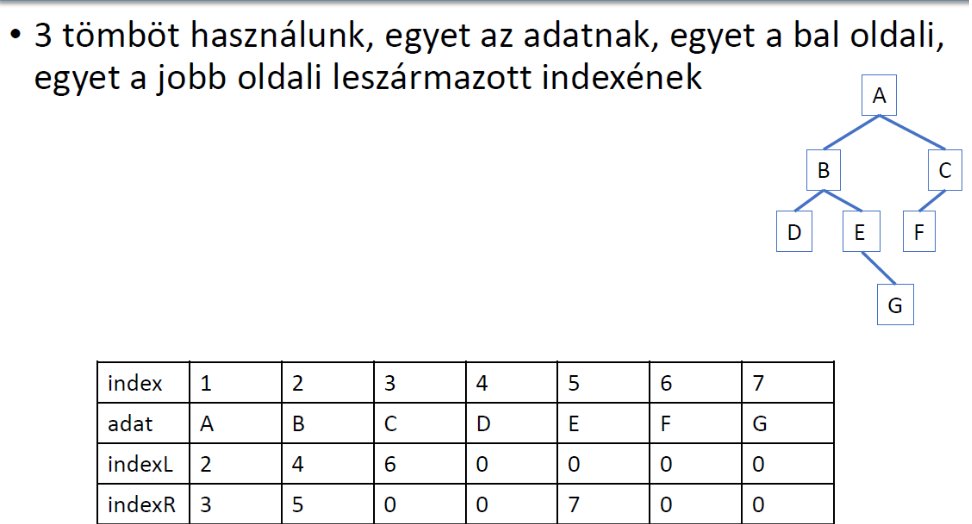
\includegraphics[scale = 0.3]{23_2.png}
                \end{center}
                \begin{center}
                    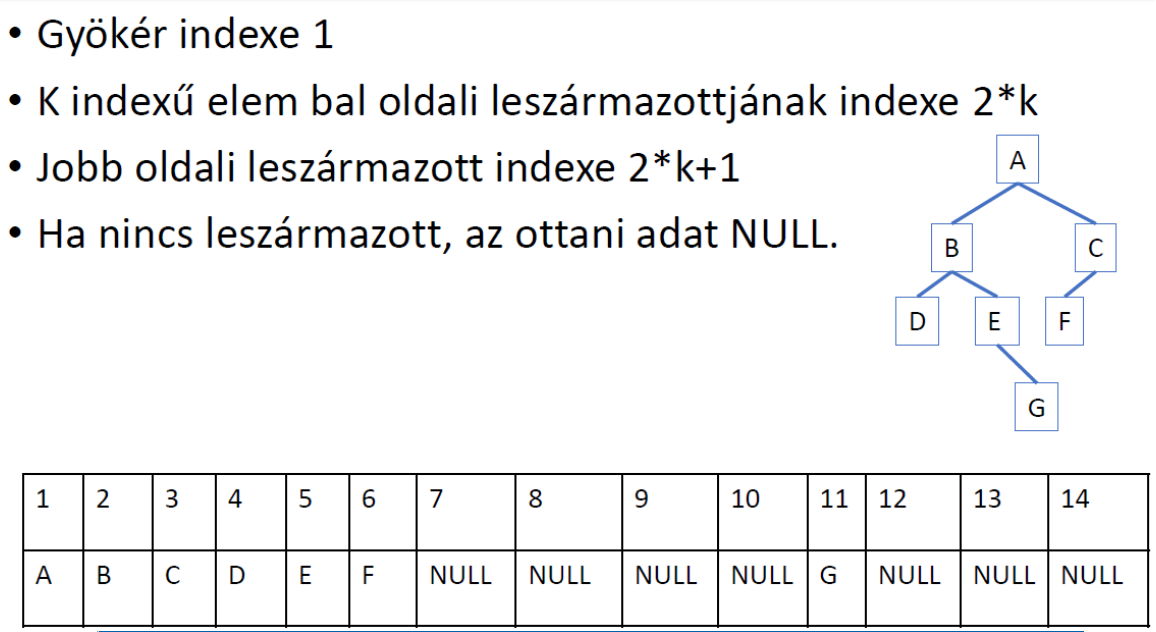
\includegraphics[scale = 0.25]{23_3.png}
                \end{center}
                \begin{center}
                    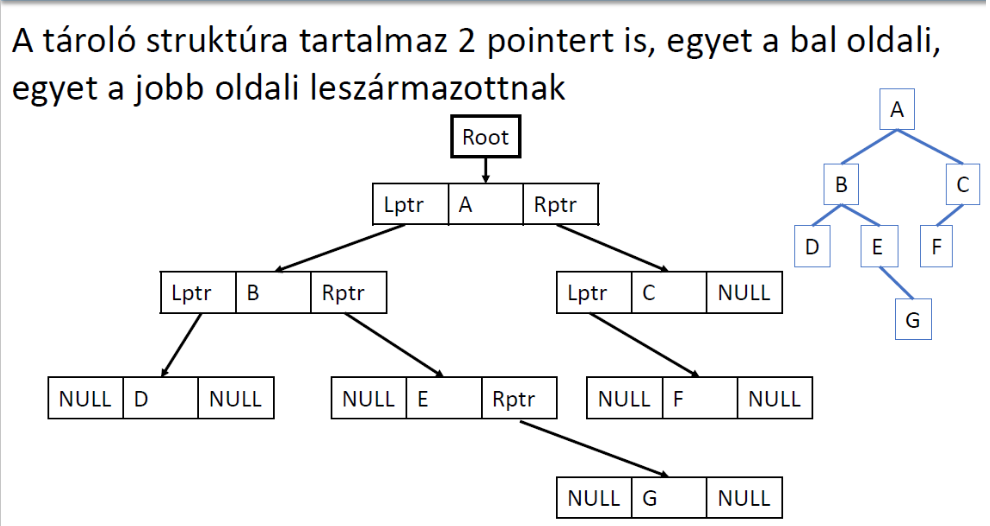
\includegraphics[scale = 0.3]{23_4.png}
                \end{center}
            \end{tcolorbox}
            
            \begin{tcolorbox}[colback=blue!5!white,colframe=blue!50!black,title= 23. Ismertesse a veremtár működését!]
                \begin{itemize}
                    \item \textbf{LIFO:} az utoljára berakott elem jön ki először (Last In First Out)
                    \item \textbf{Push:} elemet a verembe rak
                    \item \textbf{Pop:} elemet leemel a verem tetejéről
                    \item \textbf{SP:} stackpointer, a verem tetejét mutatja
                \end{itemize}
                \textbf{C nyelvű programok futása közben hol van szerepe a veremtárnak?}
                \begin{itemize}
                    \item \textbf{Alkalmazások:}
                    \begin{itemize}
                        \item függvényhívás
                        \item rekurzió
                        \item böngésző „vissza”
                        \item szövegszerkesztő „undo” gombja.
                    \end{itemize}
                \end{itemize}
            \end{tcolorbox}
            
            \begin{tcolorbox}[colback=blue!5!white,colframe=blue!50!black,title= 24. Ismertesse a sor adatszerkezet és a ciklikus buffer működését!]
                \begin{itemize}
                    \item \textbf{FIFO:} First In, First Out
                    \item Sor tárolásához 2 mutató szükséges: beírási mutató (WP), kiolvasási mutató (RP). A kiolvasási nem előzheti meg a beírásit. A mutató index is lehet a tömbelemre.
                    \item Ha WP==RP, nincs új adat a sorban. Beírás és kiolvasás előtt vagy után mutatót növelni. Az ábra az „után” szituációt mutatja.
                    \item Billentyűzet puffer, windowsesemények queue-ja.
                \end{itemize}
                \begin{center}
                    \fbox{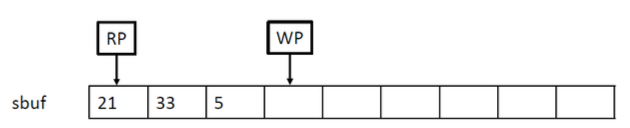
\includegraphics[scale = 0.8]{25_1.png}}
                \end{center}
                \textbf{Ciklikus Buffer:}
                \begin{itemize}
                    \item Egy speciális \textbf{queue:} a tárolásra használt tömb elfogyása után újra kezdődik az elejétől.
                    \item Tömb neve legyen sbuf, a két kétindex WP és RP
                    \item Új adat érkezése: sbuf[WP++]=adatbe; beírás
                    \item Ha WP==tömbméret, legyen WP=0;
                    \item WP!=RP esetben kiolvasás következik
                    \item Kiolvasás: adatki=sbuf[RP++];
                    \item Ha RP==tömbméret, legyen RP=0;
                    \item Ha nem olvassuk ki, akkor a régi értékek törlődnek.
                \end{itemize}
            \end{tcolorbox}
            
            \begin{tcolorbox}[colback=blue!5!white,colframe=blue!50!black,title= 25. Ismertesse számpéldával a gyorsrendezés (quick sort) algoritmust! Adja meg az algoritmus átlagos és legrosszabb komplexitását!]
                \begin{itemize}
                    \item Legyen \(S\) halmaz a rendezendő elemek halmaza
                    \item Válasszunk egy \(t\) támpont elemet.
                    \item S elemeit t kivételével két diszjunkthalmazba (\(S_1\) és \(S_2\)) soroljuk:
                    \item \(S_1 = x\in S-t \mid x\leq t\)
                    \item \(S_2 = x\in S-t \mid x > t\)
                    \item \(S_1\)-re és \(S_2\)-re rekurzívan meghívjuk a gyorsrendezést.
                    \item Eredmény: \(quicksort(S_1)+t+quicksort(S_2)\)
                    \item Amikor az összes halmaz 1 elemet tartalmaz, megállunk.
                    \item Átlagos komplexitás: \(O(n*log(n))\). Legrosszabb eset \(O(n^2)\).
                \end{itemize}
                \textbf{Példa a gyorsrendező algoritmsra a C-nyelvben:}
                \begin{Verbatim}
#include <stdio.h>
void swap(int *a, int *b) {
        int temp = *a;
        *a = *b;
        *b = temp;}           
int partition(int arr[], int low, int high) {
        int pivot = arr[high];
        int i = low - 1;  
                            
for (int j = low; j < high; j++) {
        if (arr[j] <= pivot) {
            i++;
            swap(&arr[i], &arr[j]);
        }}                    
            swap(&arr[i + 1], &arr[high]);
            return i + 1;}
                                    
void quickSort(int arr[], int low, int high) {
        if (low < high) {
            int pivotIndex = partition(arr, low, high);
                quickSort(arr, low, pivotIndex - 1);
                quickSort(arr, pivotIndex + 1, high);
        }}
            \end{Verbatim}
            \end{tcolorbox}
                                    
            \begin{tcolorbox}[colback=blue!5!white,colframe=blue!50!black,title= 26. Ismertesse az egyed-kapcsolat modellt és alábbi fogalmait: egyedtípus{,} kapcsolat- típus{,} tulajdonság!]
                                        \begin{itemize}
                                            \item \textbf{Egyedtípus (Entity type):} Az egyedek osztályát vagy kategóriáját jelöli. Az egyedtípus meghatározza, hogy az egyedek milyen tulajdonságokkal rendelkeznek és milyen kapcsolatokat tarthatnak fenn más egyedekkel. Például lehet egy "Diák" egyedtípus, amelynek tulajdonságai lehetnek a neve, életkora, osztálya stb.
                                            \item \textbf{Kapcsolat-típus (Relationship type):} Az egyedek közötti kapcsolatot jelöli. A kapcsolat-típus meghatározza, hogy az egyedek milyen módon kapcsolódnak egymáshoz. Például lehet egy "Tanul" kapcsolat-típus, amely egy diák és egy tantárgy közötti kapcsolatot reprezentál.
                                            \item \textbf{Tulajdonság (Attribute):} Az egyedek jellemzőit vagy attribútumait jelöli. A tulajdonságok konkrét információkat tárolnak az egyedekről. Például a "Diák" egyedtípusnál lehetnek olyan tulajdonságok, mint a név, életkor, osztály stb. A tulajdonságok meghatározzák az egyedek jellemzőit és értékeit.
                                        \end{itemize}
            \end{tcolorbox}
                                    
            \begin{tcolorbox}[colback=blue!5!white,colframe=blue!50!black,title= 27. Ismertesse a relációs adatbázisok felépítését és alábbi fogalmait: fokszám{,} kardinalitás{,} attribútum{,} vetítés{,} kiválasztás{,} kulcs{,} szuperkulcs{,} elsődleges kulcs{,} külső kulcs.]
                                        \begin{itemize}
                                            \item A matematikában reláción n darab halmaz \textbf{direkt szorzatának részhalmazát} értjük.
                                            \item A relációt \textbf{név}vel azonosítjuk.
                                            \item A relációban minden \textbf{sor különböző.}
                                            \item Létezik a szorzatot alkotó halmazok olyan halmaza, ami a reláció bármely elemét egyértelműen azonosítja (\textbf{kulcs})
                                            \item A szorzatot alkotó halmazok (értelmezési tartományok) száma a \textbf{reláció fokszáma}
                                            \item A reláció \textbf{elemeinek száma} a reláció \textbf{kardinalitása}
                                            \item Az egyes elemekben a tényezők konkrét értéke az \textbf{attribútum}
                                            \item \textbf{Csonkító műveletek:}
                                            \begin{itemize}
                                                \item \textbf{Vetítés (projection):} tényezők (értelmezési tartományok) kiemelése
                                                \item \textbf{Kiválasztás (select):} elemek kiválasztása
                                            \end{itemize}
                                            \item \textbf{Szuperkulcs:} a sorokat megkülönböztető oszlophalmaz
                                            \item \textbf{Kulcs:} minimális elemszámú szuperkulcs
                                            
                                            \item \textbf{Elsődleges kulcs (Primary Key):} a megkülönböztetésre választott kulcs
                                            \item \textbf{Külső kulcs (Foreign Key):} 1:N és M:N kapcsolat leírása esetén a másik tábla elsődleges kulcsa
                                        \end{itemize}
                                        
                                        
            \end{tcolorbox}
                                    
            \begin{tcolorbox}[colback=blue!5!white,colframe=blue!50!black,title= 28. Tervezzen egy relációs adatbázis-szerkezetet{,} amely M:N típusú kapcsolatot tud tárolni!]
                                        \textbf{Példa, mely tárolja egy bolt termékeinek és vásárlóinak kapcsolatát.}
                                        \begin{itemize}
                                            \item 1. Tábla: Products
                                            \begin{itemize}
                                                \item \(product_{id}\) (egyedi azonosító)
                                                \item \(product_{name}\)
                                                \item \(product_{description}\)
                                                \item egyéb tulajdonságok
                                            \end{itemize}
                                            \item 2. Tábla: Buyers 
                                            \begin{itemize}
                                                \item \(buyer_{id}\) (egyedi azonosító)
                                                \item \(buyer_{name}\)
                                                \item \(buyer_{address}\)
                                                \item egyéb adatok
                                            \end{itemize}
                                            \item 3. Kapcsolótábla: Purchases
                                            \begin{itemize}
                                                \item \(purchase_{id}\) (egyedi azonosító)
                                                \item \(buyer_{id}\) (külső kulcs a Vásárlók táblában)
                                                \item \(product_{address}\) (külső kulcs a Termékek táblában)
                                                \item egyéb adatok  (pl. vásárlás dátuma, mennyiség, ár stb.)
                                            \end{itemize}
                                        \end{itemize}
                                        A Purchases tábla a kapcsolatot tárolja a vásárlók és a termékek között. Minden sor egy adott vásárlást reprezentál, ahol a \textbf{\(buyer_{id}\)} mező a kapcsolódó vásárlót azonosítja, a \textbf{\(product_{id}\)} mező pedig a kapcsolódó terméket azonosítja. Így a Purchases tábla segítségével nyomon követhetjük, hogy melyik vásárló melyik terméket vásárolta.    
            \end{tcolorbox}
                                    
            \begin{tcolorbox}[colback=blue!5!white,colframe=blue!50!black,title= 29. Ismertesse a kernel feladatait az operációs rendszerben!]
                                        \begin{itemize}
                                            \item Folyamat kezelés (Process management)
                                            \item Memória kezelés (allokáció, felszabadítás, relokáció)
                                            \item Háttértár kezelés
                                            \item I/O rendszer kezelés
                                            \item Fájl kezelés
                                            \item Védelmi rendszer
                                            \item Hálózat elérés támogatása
                                        \end{itemize}
            \end{tcolorbox}
                                    
            \begin{tcolorbox}[colback=blue!5!white,colframe=blue!50!black,title= 30. Ismertesse a folyamatok típusait a többi folyamathoz viszonyulás alapján! ]
                                        \begin{itemize}
                                            \item \textbf{Független folyamatok:} egymás működését semmilyen módon nem befolyásolják.
                                            \item \textbf{Versengő folyamatok:} nem ismerik egymást, de közös erőforrásokon kell osztozniuk.
                                            \item \textbf{Együttműködő folyamatok:} ismerik egymást, együtt dolgoznak egy feladat megoldásán, információt cserélnek.
                                        \end{itemize}
            \end{tcolorbox}
                                    
            \begin{tcolorbox}[colback=blue!5!white,colframe=blue!50!black,title= 31. Ismertesse a folyamatok kommunikációját bináris szemafor segítségével!]
                                        \begin{itemize}
                                            \item \textbf{Vezérlés:} szemafor segítségével.
                                        \end{itemize}
                                        \begin{center}
                                            \fbox{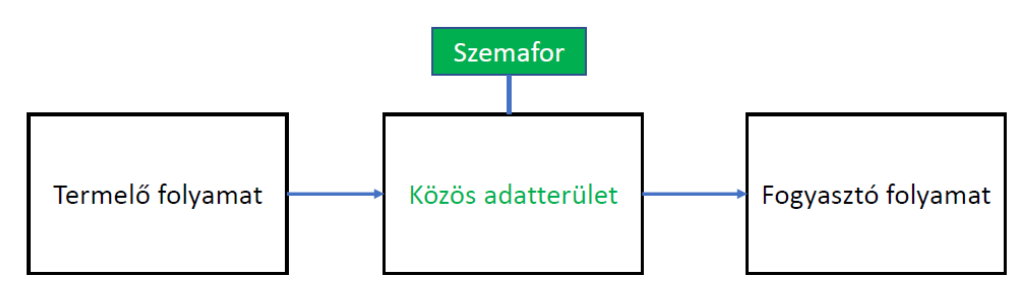
\includegraphics[scale = 0.6]{32_1.png}}
                                        \end{center}
                                        \begin{itemize}
                                            \item Mielőtt a folyamat használni kezdené a közös erőforrást, ellenőriznie kell, hogy az szabad-e. (ezt az adott közös erőforráshoz rendelt bináris szemafor jelzi.)
                                            \item Csak akkor kezdheti el használni, ha a szemafor szabadot jelzett, ellenkező esetben várakoznia kell.
                                        \end{itemize}
                                        \begin{center}
                                            \fbox{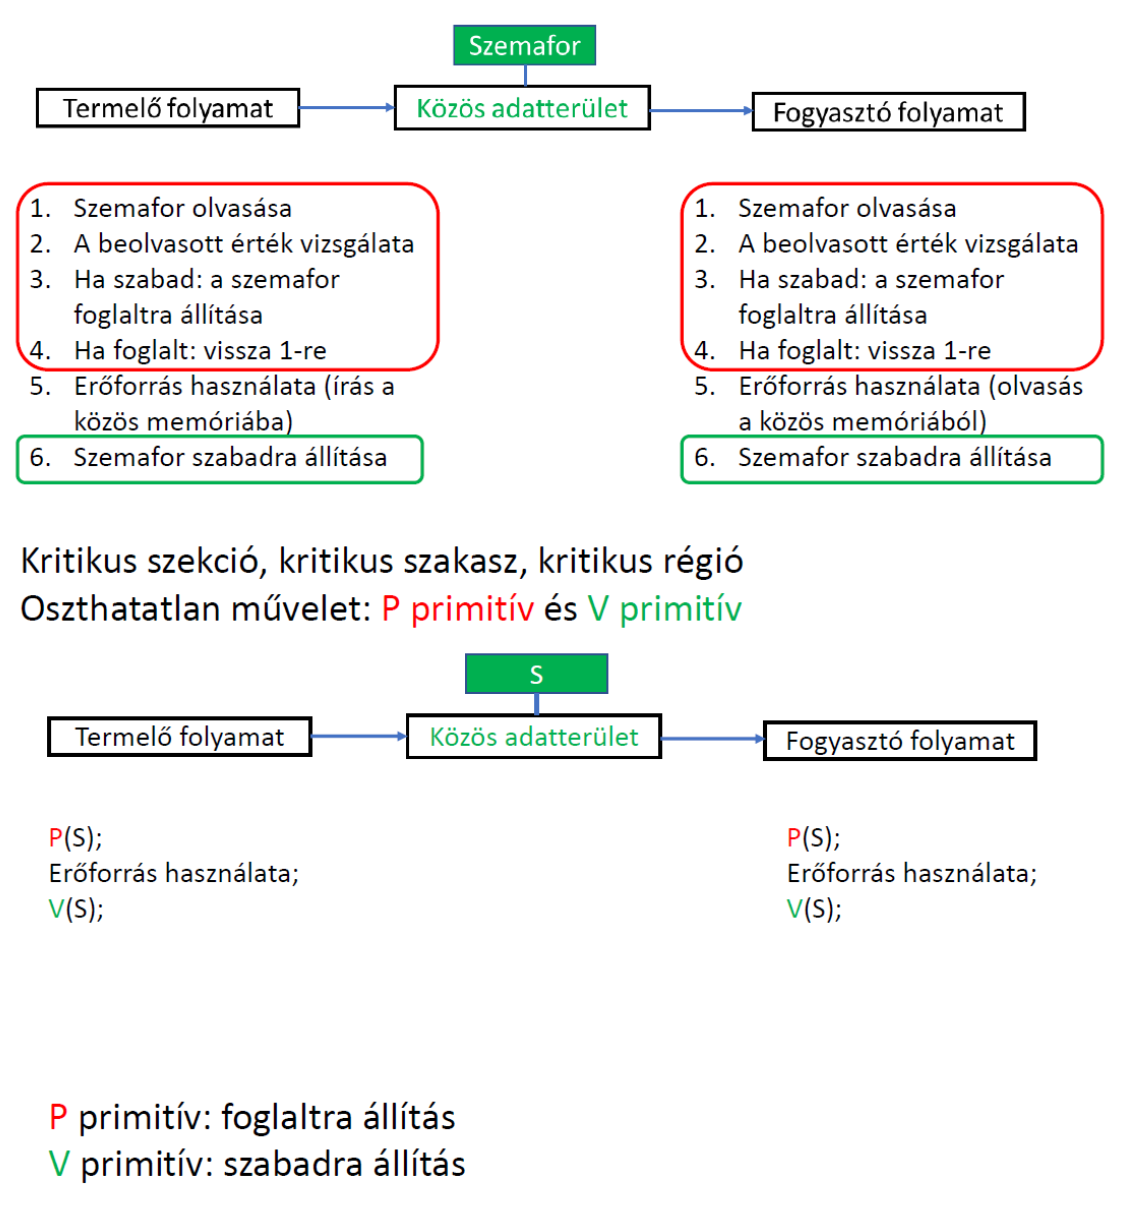
\includegraphics[scale = 0.75]{32_2.png}}
                                        \end{center}
            \end{tcolorbox}
                                    
            \begin{tcolorbox}[colback=blue!5!white,colframe=blue!50!black,title= 32. Ismertesse a folyamatok kommunikációját postaláda-kezelés esetén]
                                        \begin{itemize}
                                            \item Postaláda: olyan közös adatterület, ahová EGYNÉL TÖBB (pl. N db) üzenet írható
                                        \end{itemize}
                                        \begin{center}
                                            \fbox{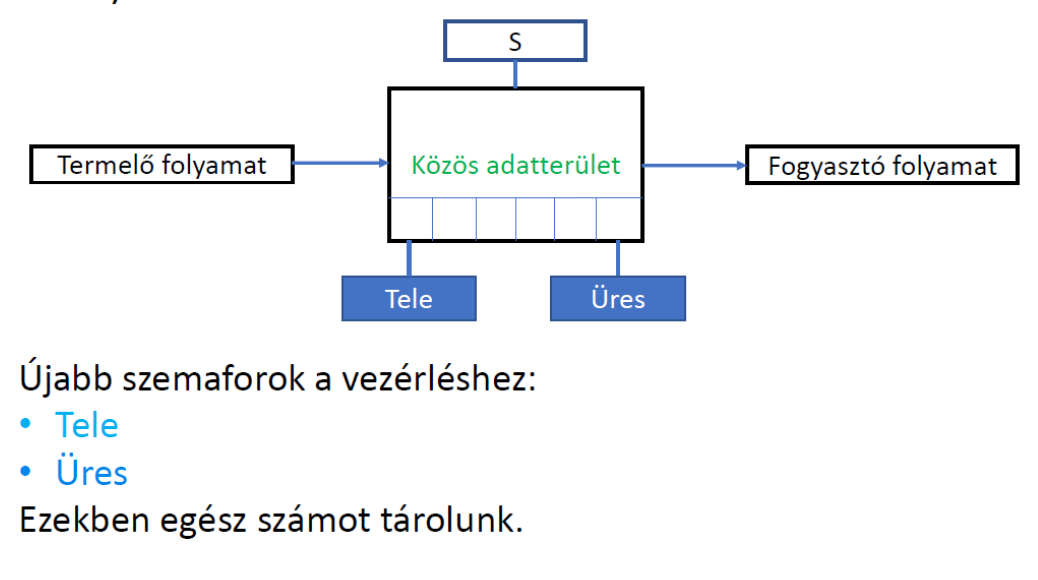
\includegraphics[scale = 0.7]{33_1.png}}                            
                                        \end{center}
                                        \begin{itemize} 
                                            \item 3 db. szemafor a vezérléséhez
                                            \item \textbf{S:} a kölcsönös kizárást megvalósító szemafor (bináris; 0=\textcolor{red}{foglalt}; 1=\textcolor{green}{szabad}; kezdeti értéke: szabad)
                                            \item \textbf{Tele:} a tele helyek száma (nem bináris; értéke 0 és N között lehet; kezdeti értéke:0)
                                            \item \textbf{Üres:} az üres helyek száma (nem bináris; értéke 0 és N között lehet; kezdeti értéke:N)
                                            \item \textcolor{red}{\textbf{P primitív:}} a paraméterül kapott szemafor értékének EGGYEL CSÖKKENTÉSE (bináris szemafor esetén ez a \textcolor{red}{\textbf{FOGLALTTÁ}} ÁLLÍTÁS)
                                            \item \textcolor{green}{\textbf{V primitív:}} a paraméterül kapott szemafor értékének EGGYEL NÖVELÉSE (bináris szemafor esetén ez a \textcolor{green}{\textbf{SZABADDÁ}} ÁLLÍTÁS)
                                        \end{itemize}
                                        \begin{center}
                                            \fbox{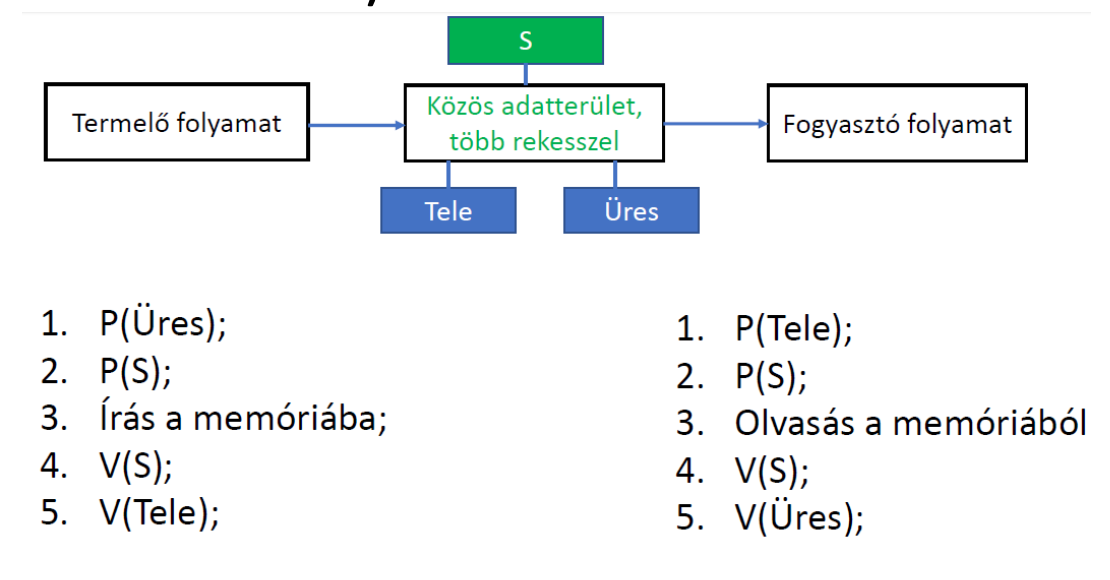
\includegraphics[scale = 0.7]{33_2.png}}                            
                                        \end{center}
            \end{tcolorbox}
                                    
            \begin{tcolorbox}[colback=blue!5!white,colframe=blue!50!black,title= 33. Ismertesse példával a bankár algoritmust!]
                                        \begin{itemize}
                                            \item Biztonságosan tervezett az a folyamatokat és erőforrásokat tartalmazó rendszer, amelyben létezik a folyamatoknak (legalább egy) olyan sorrendje, amely szerint végrehajtva őket, azok maximális erőforrás igénye is kielégíthető.
                                            \item A biztonságos rendszerben nem lehetséges holtpont kialakulása.
                                            \item Az ellenőrzést a bankár algoritmussal végezzük folyamat indítás és erőforrás foglalás előtt.
                                        \end{itemize}
                                        
                                        \begin{center}
                                            \fbox{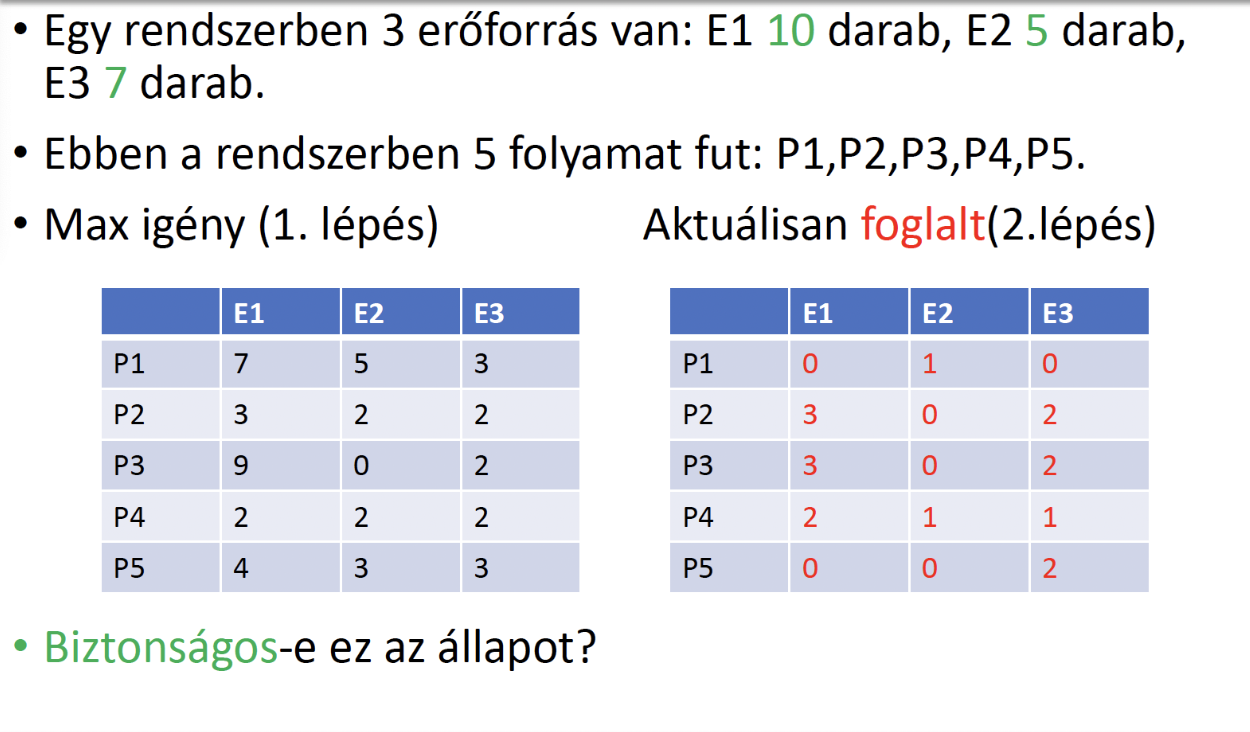
\includegraphics[scale = 0.2]{34_1.png}}                            
                                        \end{center}
                                        \begin{center}
                                            \fbox{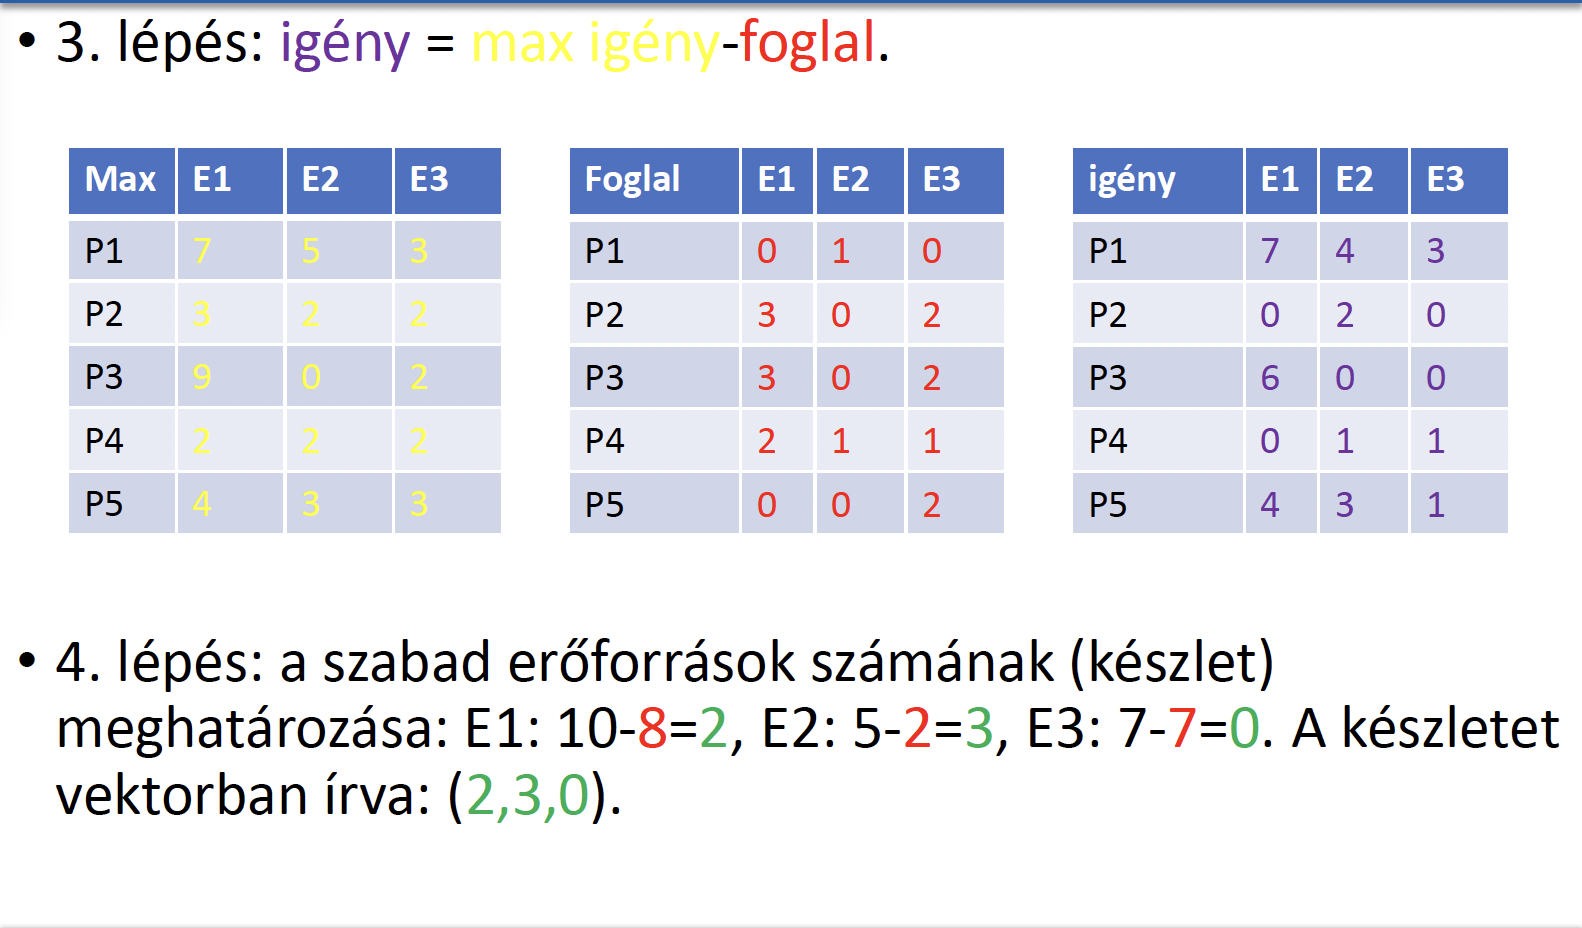
\includegraphics[scale = 0.2]{34_2.png}}                            
                                        \end{center}
                                        \begin{center}
                                            \fbox{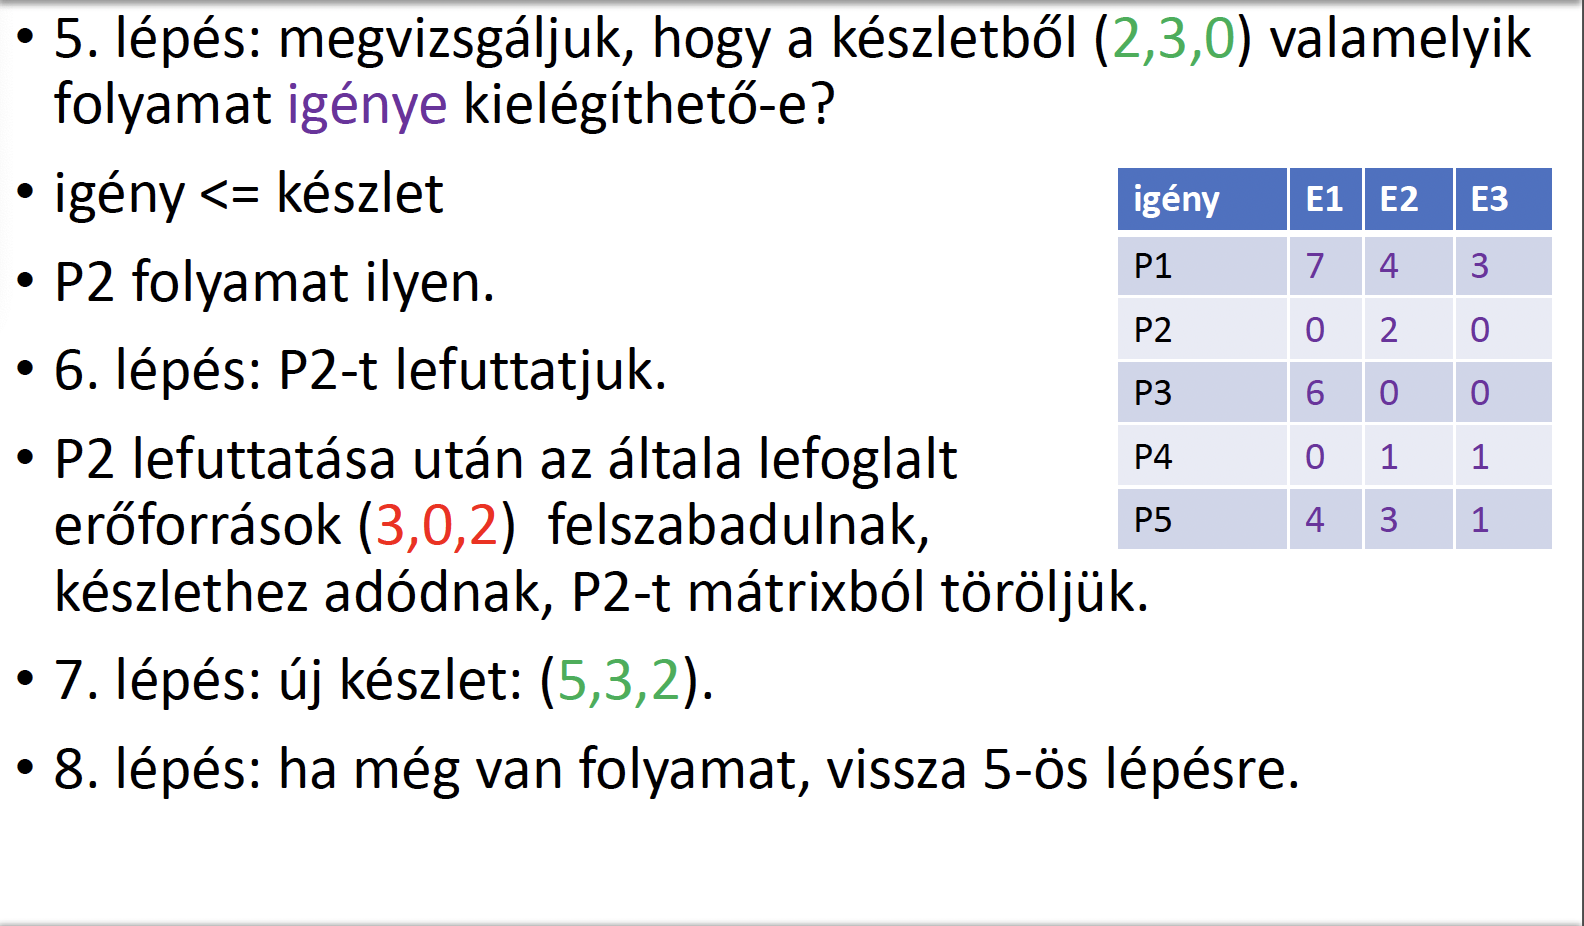
\includegraphics[scale = 0.2]{34_3.png}}                            
                                        \end{center}
                                        \begin{center}
                                            \fbox{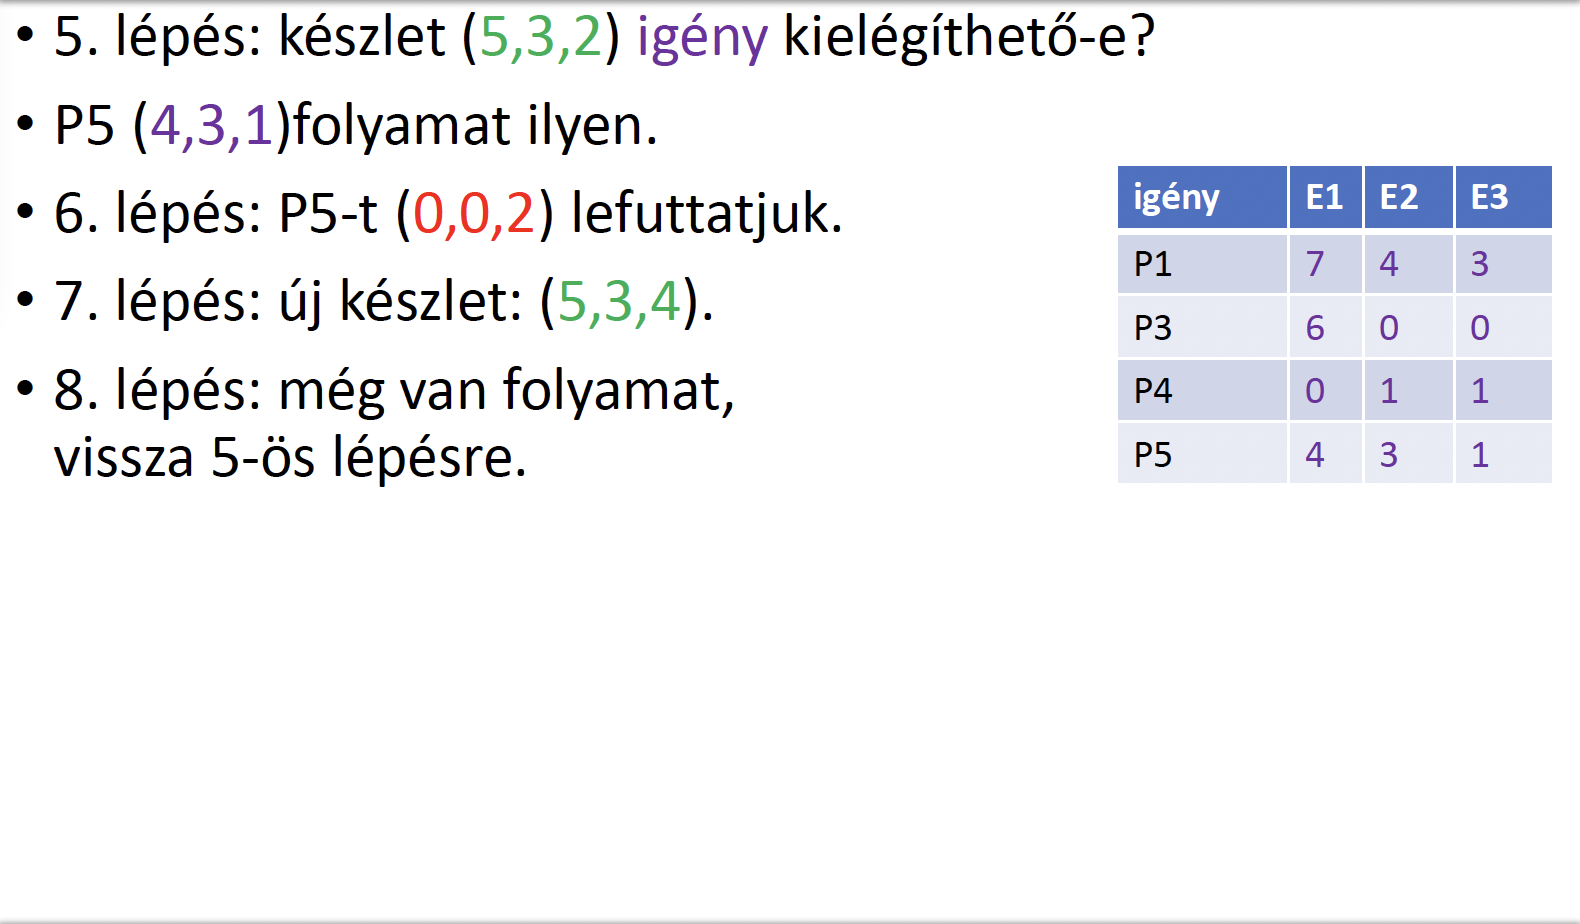
\includegraphics[scale = 0.2]{34_4.png}}                            
                                        \end{center}
                                        \begin{center}
                                            \fbox{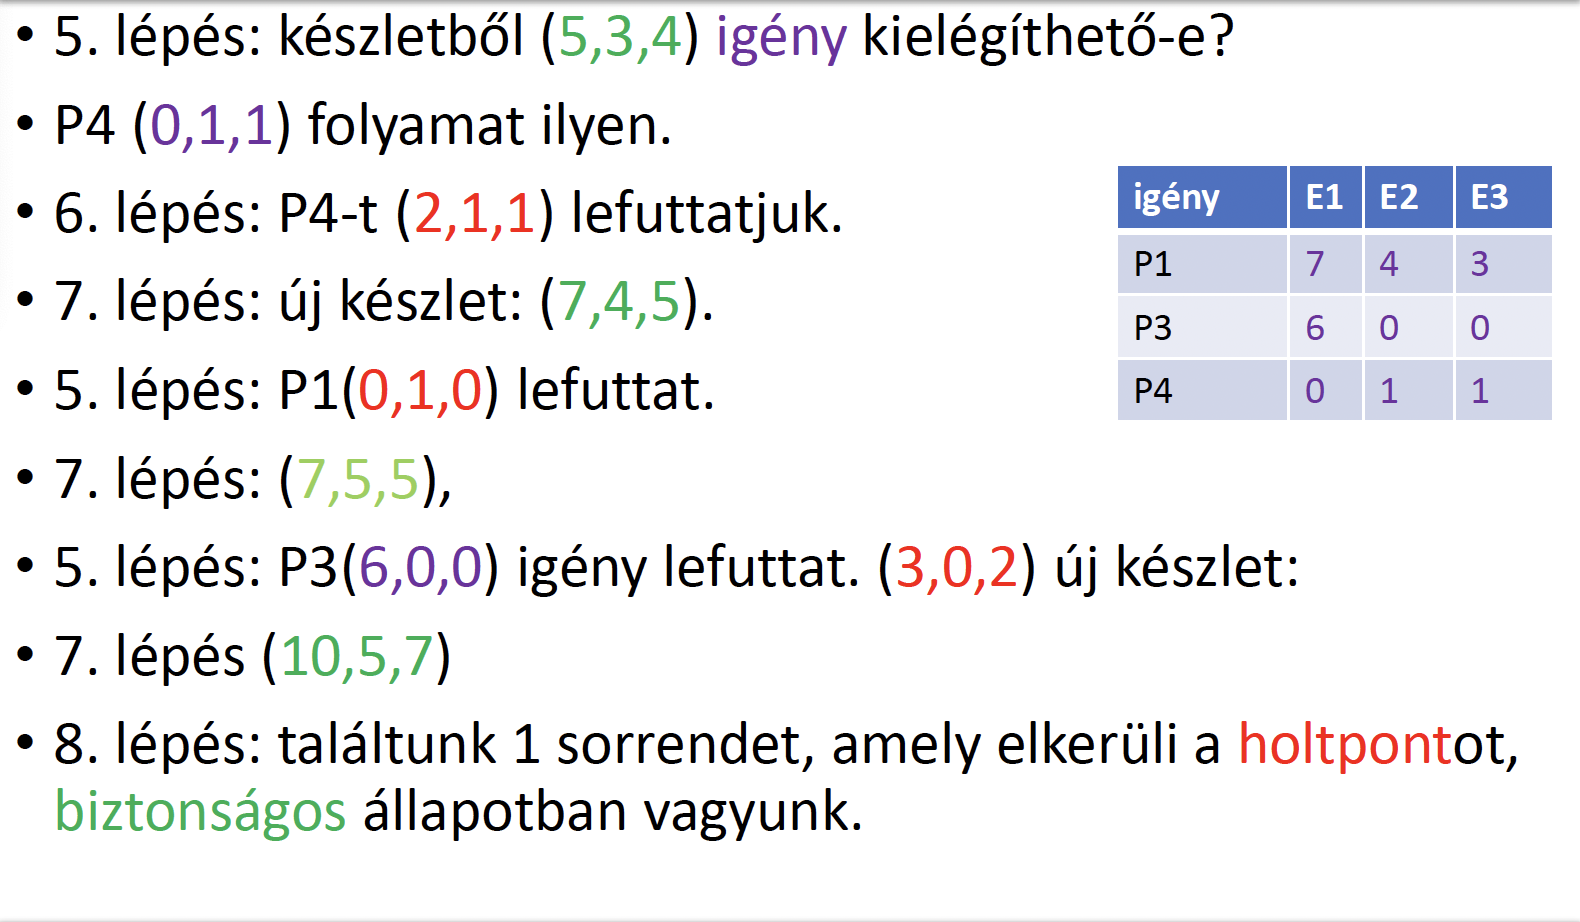
\includegraphics[scale = 0.2]{34_5.png}}                            
                                        \end{center}
            \end{tcolorbox}
                                    
            \begin{tcolorbox}[colback=blue!5!white,colframe=blue!50!black,title= 34. Ismertesse az operációs rendszerek feladat-ütemezési algoritmusait!]
                                        Többfeladatos operációs rendszerben a folyamatok közti átkapcsolást végzik.\\    
                                        \textbf{Alap algoritmusok:}
                                        \begin{itemize}
                                            \item FCFS (First Come First Served) előbb jött, előbb fut. Egyszerű, érkezési időtől függ, egy hoszú folyamat a többieket megfogja (kamion hatás)
                                            \item SJF (Shortest Job First) előbb a legrövidebb fut. Legrövidebb várakozás, előre tudni kell a lefutási időt, hosszú folyamat később kerül sorra (kiéheztetés)
                                            \item RR (Round Robin) időosztásos.
                                            \begin{itemize}
                                                \item A folyamatokat körbe szervezzük, minden folyamat csak egy időszeletet kap, lejárta után elveszi tőle az OS a vezérlést.
                                                \item Előbb is visszaadhatja, ha éppen nincs dolga.
                                                \item Prioritással kombinálható, ekkor egy prioritási szintnek saját köre van.
                                                \item Egyszerű algoritmus, nincs kiéheztetés.
                                                \item Időszelet lejártakor állapot mentés, kör újra odaértekor visszaállítás (idő).
                                                \item Idle folyamat (unix): egy kör végén már nincs folyamat, amelyet végre kellene hajtani.
                                            \end{itemize}
                                        \end{itemize}
                                        \begin{center}
                                            \fbox{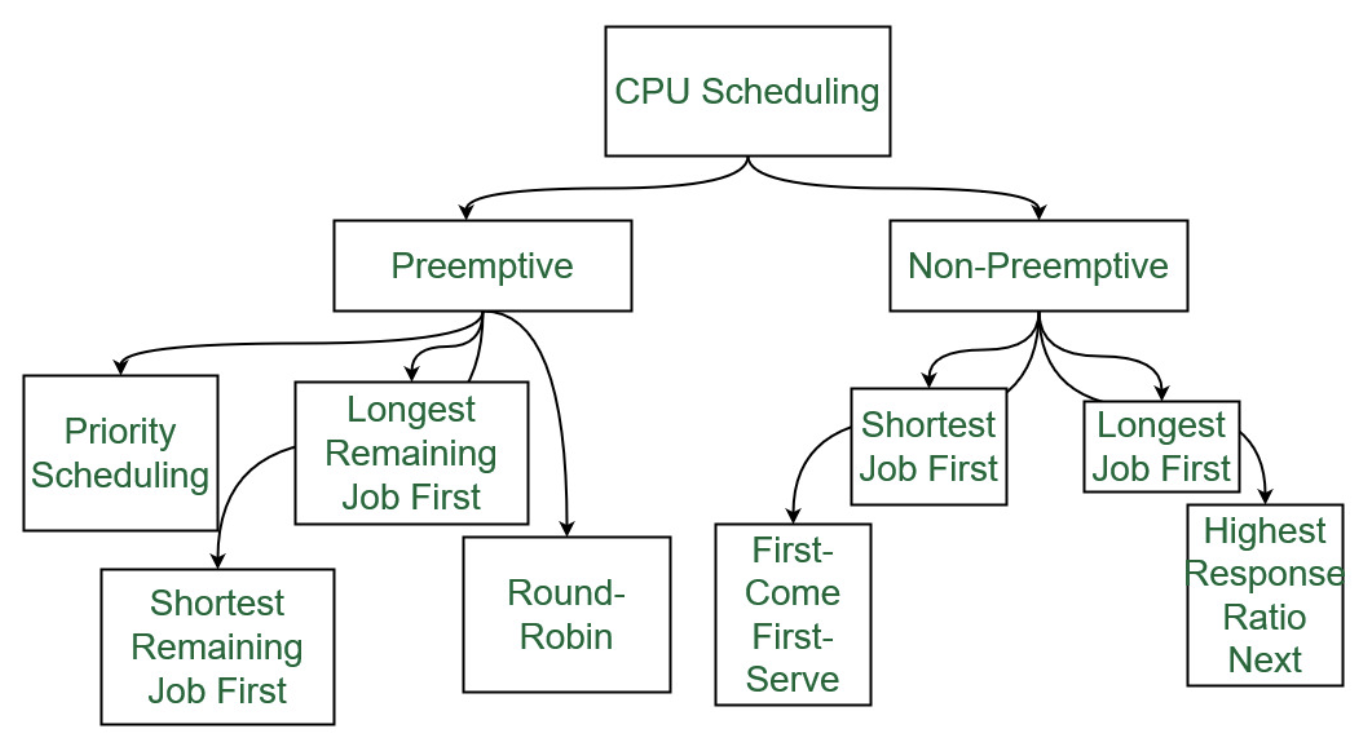
\includegraphics[scale = 0.5]{34.png}}                            
                                        \end{center}
            \end{tcolorbox}
                                    
            \begin{tcolorbox}[colback=blue!5!white,colframe=blue!50!black,title= 35. Ismertesse a C nyelvű forráskód fordítási és futtatási folyamatát!]
                                        \begin{center}
                                            \fbox{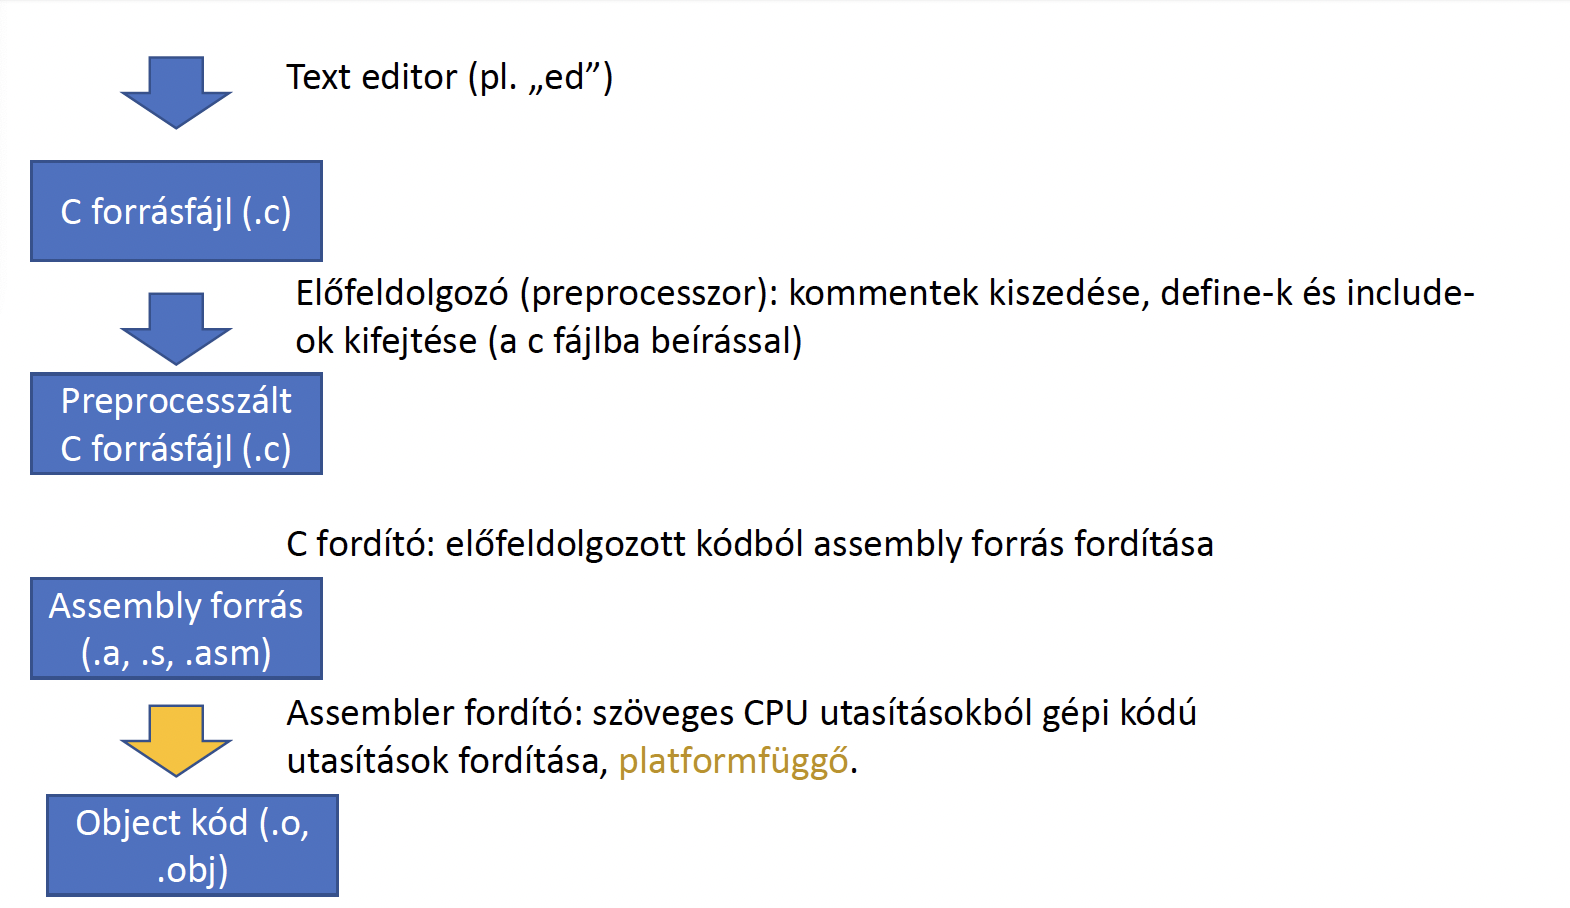
\includegraphics[scale = 0.5]{36_1.png}}                            
                                        \end{center}
                                        \begin{center}
                                            \fbox{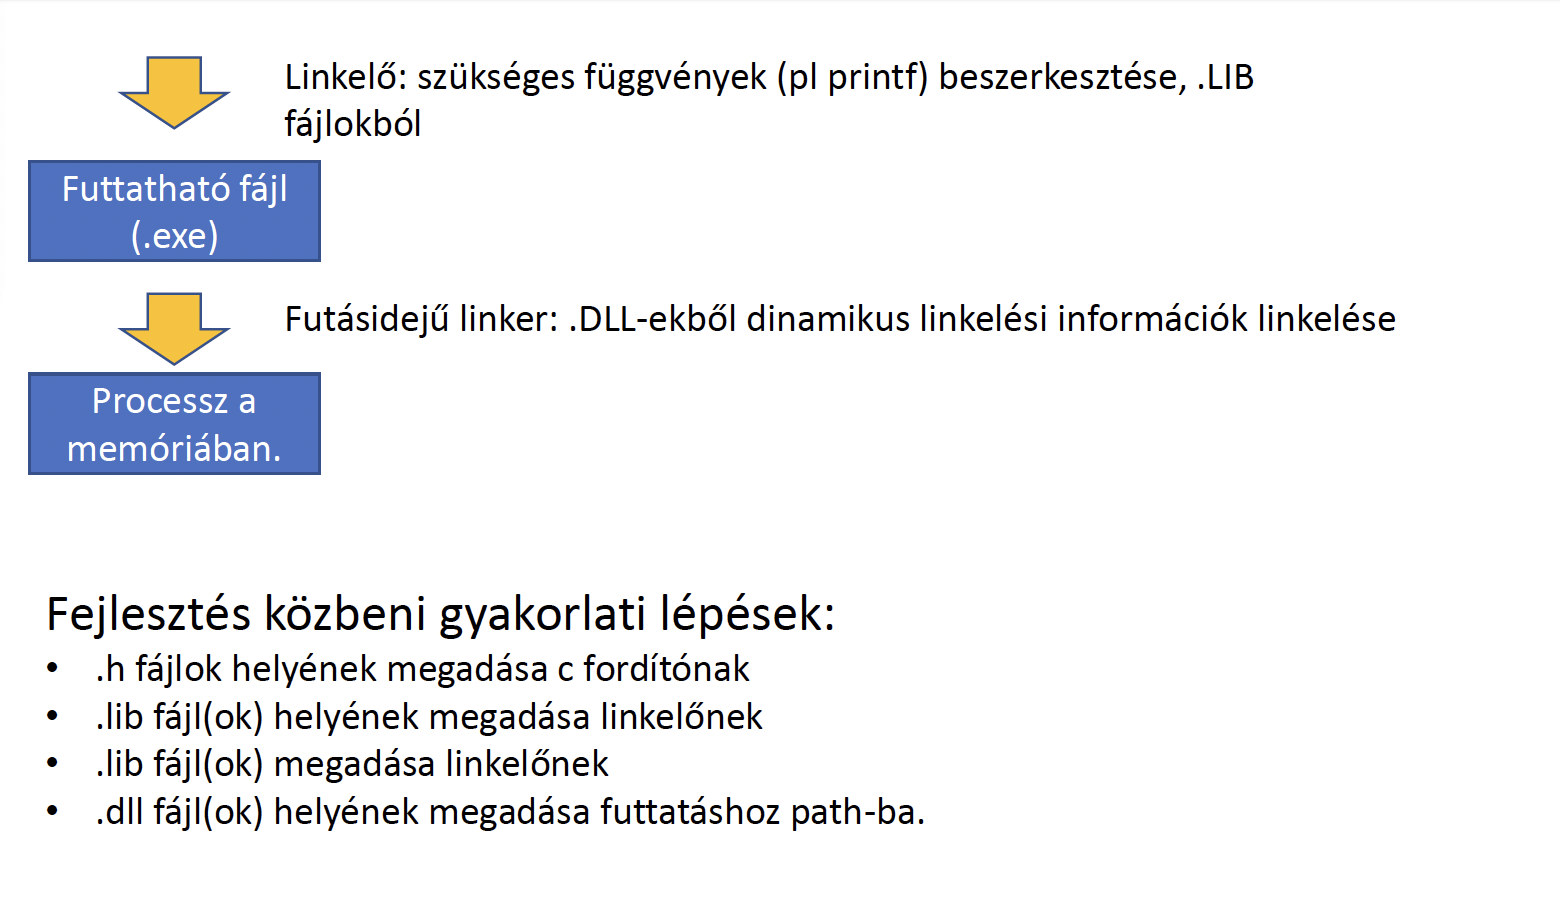
\includegraphics[scale = 0.5]{36_2.png}}                            
                                        \end{center}
            \end{tcolorbox}
                                    
            \begin{tcolorbox}[colback=blue!5!white,colframe=blue!50!black,title= 36. Ismertesse a UNIX file-elérési jogok oktális kódolását!]
                                        A UNIX file-elérési jogok oktális kódolása három számjeggyel történik, ahol minden számjegy a jogosultságok egy csoportját reprezentálja. Az oktális számjegyeket 0-tól 7-ig lehet használni, és a következő jelentéseik vannak:\\
                                        \textbf{1. Az első számjegy a tulajdonos jogait reprezentálja}    
                                        \begin{itemize}
                                            \item 0: Nincs jogosultság
                                            \item 1: Csak végrehajtási jog
                                            \item 2: Csak írási jog
                                            \item 3: Írási és végrehajtási jog
                                            \item 4: Csak olvasási jog
                                            \item 5: Olvasási és végrehajtási jog 6: Olvasási és írási jog
                                            \item 6: Olvasási ás írási jog
                                            \item 7: Olvasási, írási és végrehajtási jog
                                        \end{itemize}
                                        \textbf{2. A második számjegy a csoport jogait reprezentálja.}
                                        \begin{itemize}
                                            \item Az értékek megegyeznek az első számjegy jelentéseivel.
                                        \end{itemize}
                                        \textbf{3. A harmadik számjegy a többi felhasználó jogait reprezentálja.}
                                        \begin{itemize}
                                            \item Az értékek megegyeznek az első számjegy jelentéseivel.
                                        \end{itemize}
                                        \textbf{Példa:} jogosultságokat össze lehet adni a megfelelő számjegyekkel. Például, ha a tulajdonosnak olvasási, írási és végrehajtási jogai vannak (7), a csoportnak csak olvasási és végrehajtási jogai vannak (5), és a többi felhasználónak csak végrehajtási joga van (1), akkor a jogokat az oktális kódolásban a következőképpen reprezentálhatjuk: 751\\
                                        \begin{center}
                                            \fbox{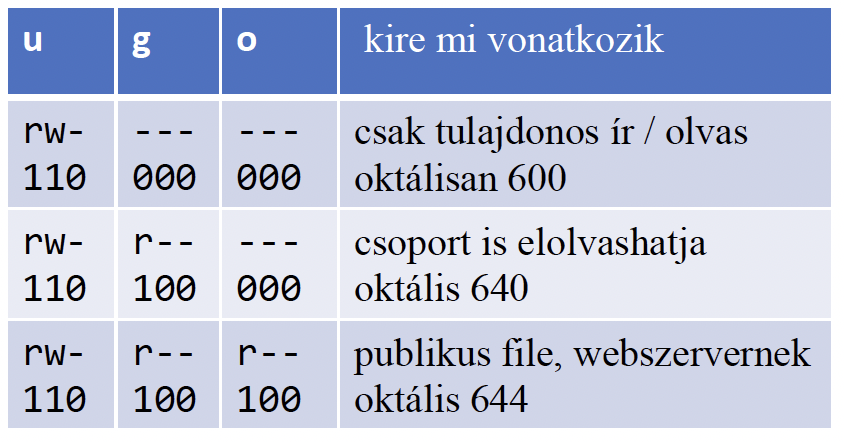
\includegraphics[scale = 0.9]{36_3.png}}
                                        \end{center}
            \end{tcolorbox}
                                    
            \begin{tcolorbox}[colback=blue!5!white,colframe=blue!50!black,title= 37. Ismertesse a hírközlés Shannon-féle modelljét a modellben található egységek funkciójának leírásával!]
                                        A hírközlés során egy üzenetet juttatunk el térben és/vagy időben másik pontra.
                                        \begin{center}
                                            \fbox{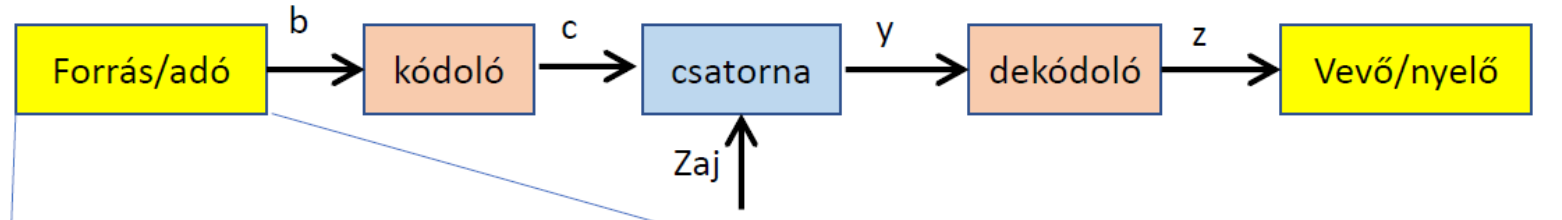
\includegraphics[scale = 0.5]{38_1.png}}                            
                                        \end{center}
                                        \begin{enumerate}
                                            \item \textcolor{red}{\textbf{Adatkészlet:}} Az eredeti üzenet vagy adat, amit továbbítani szeretnénk.
                                            \item \textcolor{red}{\textbf{Forráskódolás:}} Az adatkészlet hatékonyabb formába való átalakítása a tárolás és továbbítás céljából.
                                            \item \textcolor{red}{\textbf{Kódolás:}} Az adatok kódolása a zajállóság és hibajavítás érdekében.
                                            \item \textcolor{red}{\textbf{Csatorna:}} A közeg, amelyen keresztül az adatok továbbításra kerülnek.
                                            \item \textcolor{red}{\textbf{Zaj:}} A zavaró hatás, amely befolyásolja az adatok továbbítását és értelmezését.
                                            \item \textcolor{red}{\textbf{Dekódolás:}} A csatornakódolt adatok visszaalakítása az eredeti formába.
                                            \item \textcolor{red}{\textbf{Végpont(Vevő/Nyelő):}} A kommunikáció résztvevőinek végpontjai, ahol az adatok fogadása és továbbítása történik.
                                        \end{enumerate}
            \end{tcolorbox}
                                    
            \begin{tcolorbox}[colback=blue!5!white,colframe=blue!50!black,title= 38. Ismertesse az információ mennyiség Hartley-féle és Shannon-féle meghatározását!]
                                        Az információvalamely véges számú, előre ismert esemény közül annak megnevezése, hogy melyik következett be.   
                                        \begin{itemize} 
                                            \item \textcolor{red}{\textbf{Hartley:}} m számú, azonos valószínűségű esemény közül egy megnevezésével nyert információ: \(I =log_2m\)
                                            \item \textcolor{red}{\textbf{Shannon:}} minél váratlanabb egy esemény, bekövetkezése annál több információt jelent.
                                        \end{itemize}
            \end{tcolorbox}
                                    
            \begin{tcolorbox}[colback=blue!5!white,colframe=blue!50!black,title= 39. Ismertesse számpéldával a Huffman-kódolást!]
                                        A legrövidebb átlagos szóhosszúságú prefix kód.
                                        \begin{enumerate}
                                            \item Valószínűségek szerint sorba rendezia forrásszimbólumokat.
                                            \item A két legkisebb valószínűségű szimbólumot összevonja. Az összevont „szimbólum” valószínűsége a két másik összege.
                                            \item Az 1-2 lépést addig ismétli, amíg egy darab, 1 valószínűségű szimbólum marad.
                                            \item A kapott gráf minden csomópontja előtti két élt megcímkézi 0-val és 1-gyel: ez lesz a kódfa. Bináris fa.
                                            \item A kódfa gyökerétőlelindulva megkeresi az adott szimbólumhoz tartozó útvonalat, kiolvassa az éleknek megfelelő biteket. A kapott bitsorozatot rendeli a szimbólumhoz kódszóként.
                                        \end{enumerate}
                                        \begin{center}
                                            \fbox{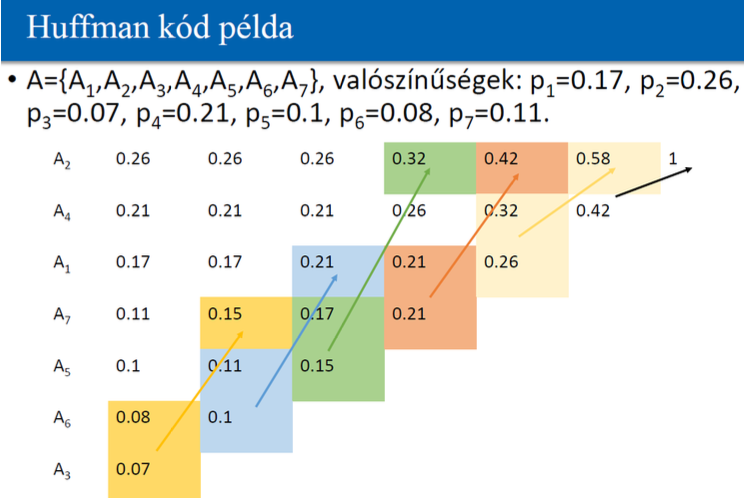
\includegraphics[scale = 0.65]{40_1.png}}                            
                                        \end{center}
                                        
            \end{tcolorbox}
                                    
            \begin{tcolorbox}[colback=blue!5!white,colframe=blue!50!black,title= 40. Ismertessen fizikai és logikai hálózati topológiákat!]
                                        \textbf{Fizikai hálózati topológiák:}    
                                        \begin{enumerate}
                                            \item \textbf{Busz topológia:} Az eszközök egy közös adatbuszon vannak összekapcsolva. Az adatokat az adatbuszon továbbítják, és az összes eszköz figyeli a buszt. Az adatok mindkét irányban közösek a buszon.
                                            \item \textbf{Gyűrű topológia:} Az eszközök egy körforgásban vannak elrendezve, és az adatok körforgásszerűen továbbítódnak az eszközök között. Minden eszköz fogadja és továbbítja az adatokat.
                                            \item \textbf{Csillag topológia:} Az eszközök központi csomópontra (switch vagy hub) vannak csatlakoztatva. Az adatok a csomóponton keresztül továbbítódnak az eszközök között.
                                            \item \textbf{Fa topológia:} Az eszközök fa szerkezetben vannak elrendezve, ahol a központi csomópontok csatlakoznak az alsó szintű eszközökhöz. Az adatok a fa struktúrán keresztül továbbítódnak.
                                        \end{enumerate}
                                        \begin{center}
                                            \fbox{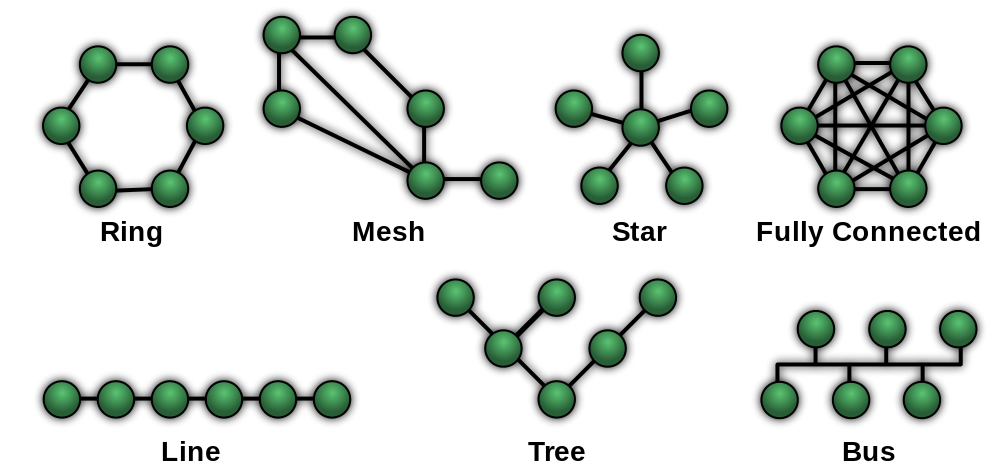
\includegraphics[scale = 0.4]{41_1.png}}                            
                                        \end{center}
                                        \textbf{Logikai hálózati topológiák:}
                                        \begin{enumerate}
                                            \item \textbf{Csillag topológia:} Az eszközök központi csomópontra vannak csatlakoztatva, de a kommunikáció közvetlenül a csomóponton keresztül történik.
                                            \item \textbf{P2P (peer-to-peer) topológia:} Az eszközök közvetlenül egymással vannak összekapcsolva, és közvetlenül kommunikálnak egymással anélkül, hogy központi csomópontot használnának.
                                            \item \textbf{Hierarchikus topológia:} Az eszközök hierarchiában vannak szervezve, ahol van egy központi csomópont, amely összekapcsolja az alsóbb szintű csomópontokat.
                                            \item \textbf{Mesh topológia:} Az eszközök közvetlenül egymással vannak összekapcsolva, és több út áll rendelkezésre az adatok továbbításához. Ez a topológia magas redundanciát és megbízhatóságot biztosít.
                                        \end{enumerate}
                                        \textbf{Melyik hálózati elsőbbségi elvhatékony egy kis terhelésű és egy nagy terhelésű hálózaton?}
                                        \begin{itemize}
                                            \item \textbf{Kis terhelésű hálózaton:} Az arányos elosztás vagy fair share elve hatékony. Ez az elv az erőforrásokat egyenlően osztja szét az eszközök vagy felhasználók között, így mindenki azonos feltételekkel érheti el a rendelkezésre álló erőforrásokat.
                                            \item \textbf{Nagy terhelésű hálózaton:} A prioritás alapú elv hatékony. Ebben az esetben bizonyos forgalom vagy szolgáltatások kapnak előnyt a többi forgalommal szemben. Ez lehetővé teszi a kritikus feladatok gyorsabb és megbízhatóbb végrehajtását a nagy terhelésű környezetben.
                                        \end{itemize}
            \end{tcolorbox}
                                    
            \begin{tcolorbox}[colback=blue!5!white,colframe=blue!50!black,title= 41. Ismertesse az ethernet hálózaton használt eszközöket!]  
                                        \begin{itemize}
                                            \item \textbf{Számítógép:} A számítógépek az ethernet hálózatok alapvető részei, amelyek csatlakoznak a hálózati infrastruktúrához és kommunikálnak más eszközökkel.
                                            \item \textbf{Switch:} A switch (kapcsoló) az ethernet hálózat központi eszköze, amely összekapcsolja a számítógépeket és más eszközöket a hálózaton belül, és csomagokat továbbít a megfelelő célállomásokhoz.
                                            \item \textbf{Router:} A router (útválasztó) a hálózatok közötti adatforgalmat irányítja és továbbítja. Az ethernet hálózaton a router a hálózatok közötti kapcsolatot biztosítja.
                                            \item \textbf{Modem:} A modem lehetővé teszi az internet-hozzáférést az ethernet hálózaton keresztül. Átalakítja az analóg jeleket digitális formátumba, és fordítva.
                                            \item \textbf{Hub:} A hub (központi elosztó) az adatokat egy portról minden másik portra továbbítja. Azonban a hub nem tudja figyelni és különbséget tenni a címzett eszközök között, ami korlátozza a hálózati teljesítményt.
                                            \item \textbf{Media converter:} A media converter (közvetítő) lehetővé teszi a különböző hálózati médiumok (például réz és optikai kábel) közötti átalakítást és összekapcsolást.
                                        \end{itemize}
                                        \textbf{Hogy védi ki a zavarokat a csavartérpár?}
                                        \begin{itemize}
                                            \item \textbf{Crossover elrendezés:} A csavart érpárokban a vezetékek páronként keresztezik egymást, így minimalizálva a zavarok befolyását a jelekre.
                                            \item \textbf{Párhuzamos vezetékek:} A csavart érpárok párhuzamos elhelyezése a kábelben segít minimalizálni a zavarokat, mivel a különböző párokban áramló jelek egymástól távolabb vannak.
                                            \item \textbf{Árnyékolás:} A csavart érpárok kábeleit általában árnyékolják, hogy csökkentsék a külső elektromágneses interferenciát.
                                            \item \textbf{A földelés szerepe:} A csavart érpárok földelése további védelmet nyújt a zavarok ellen, mivel a földelés lehetővé teszi a nem kívánt elektromos energiák levezetését.
                                        \end{itemize}
                                        \begin{center}
                                            \fbox{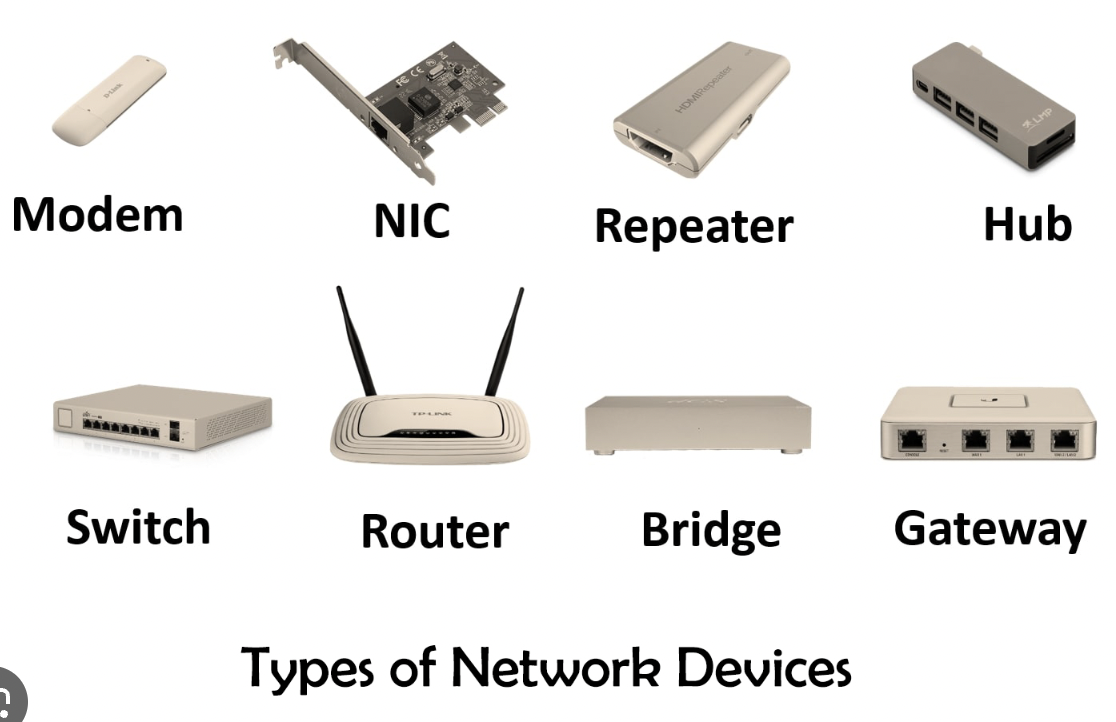
\includegraphics[scale = 0.6]{41.png}}                            
                                        \end{center}
                                        
            \end{tcolorbox}
            
            \begin{tcolorbox}[colback=blue!5!white,colframe=blue!50!black,title= 42. Ismertesse az internetes címek maszkolási algoritmusát!]
                \begin{itemize}
                    \item \textbf{IP-cím:} Az IPv4 protokoll használ 32 bites IP-címeket, amelyeket négy oktettre osztanak fel (pl. 192.168.0.1).
                    \item \textbf{Hálózati maszk:} A hálózati maszk meghatározza, hogy az IP-cím hálózati része hogyan van elkülönítve a hoszt résztől. Pl. 255.255.255.0 jelenti, hogy az első három oktett a hálózat, az utolsó oktett pedig a hoszt része.
                    \item \textbf{AND művelet:} Az IP-cím és a hálózati maszk bitjeit az AND művelettel kombinálják, hogy meghatározzák az adott IP-cím hálózati részét. Pl. 192.168.0.1 AND 255.255.255.0 = 192.168.0.0, a hálózat címe.
                    \item \textbf{Címek osztályozása:} Az IP-cím első néhány bitje meghatározza az IP-cím osztályát (A, B, C stb.), ami alapján a hálózati maszkot is meghatározzák.
                    \item Az IP-címek maszkolása lehetővé teszi a hálózati és hoszt részek elkülönítését 
                \end{itemize}    
                \textbf{Mire használható a maszkolás?}
                \begin{itemize}
                    \item \textbf{IP-címek osztályozása:} Az IP-címeket maszkolással osztályokba vagy alcsoportokba lehet sorolni, ami segíti az internetes forgalom irányítását és hálózati felépítést.
                    \item \textbf{Alhálózatok létrehozása:} A maszkolás lehetővé teszi, hogy egy nagyobb hálózatot kisebb alhálózatokra osszunk fel, ami hatékonyabb hálózati erőforrásfelhasználást és forgalomkezelést eredményez.
                    \item \textbf{Hálózati szegmentálás:} A maszkolás segít a hálózatok fizikai vagy logikai szegmentálásában, amely javítja a hálózati teljesítményt, biztonságot és skálázhatóságot.
                    \item \textbf{Hozzáférés-szabályozás:} A maszkolás lehetőséget nyújt hálózati hozzáférés-szabályozásra, hogy csak bizonyos IP-címrészek vagy alcsoportok kommunikálhassanak egymással.
                \end{itemize}
                \textcolor{red}{\textbf{A maszkolásnak fontos az IP-hálózatok hatékony tervezésében, kezelésében és biztonságában.}}
            \end{tcolorbox}
            
            \begin{tcolorbox}[colback=blue!5!white,colframe=blue!50!black,title= 43. Ismertesse a NAT (Network Address Translator) eszközt használatát az internethez való kapcsolódásban!]
                \begin{itemize}
                    \item \textbf{Privát IP-címek:} Az otthoni vagy vállalati hálózatokon belül az eszközök privát IP-címeket használnak, amelyek nem egyediek a globális interneten.
                    \item \textbf{Közös IP-cím:} A NAT-eszköz az internetre kapcsolódó privát hálózatokat egy közös IP-cím alatt reprezentálja.
                    \item \textbf{IP-cím átírás}: Amikor a privát hálózatról egy eszköz csatlakozik az internetre, a NAT-eszköz átírja az IP- címet a közös IP-címre, és megjegyzi a kapcsolódó portszámot.
                    \item \textbf{Válaszok visszirányítása:} Amikor az internetről érkezik válasz a kapcsolat kérelmére, a NAT-eszköz a portszám alapján visszairányítja a választ a megfelelő privát IP-címre és portra.
                    \item \textbf{Többes kapcsolatkezelés:} A NAT-eszköz lehetővé teszi több eszköz számára, hogy ugyanazon a közös IP- címen keresztül kommunikáljon az interneten, ami csökkenti az IP-címek szükségességét.
                    \item A NAT-eszköz használata lehetővé teszi, hogy a privát hálózatok több eszköze is kapcsolódhasson az internethez egy korlátozott mennyiségű közös IP-cím alatt. Ez növeli az internetes kapcsolat kihasználtságát és biztosítja az eszközök hálózati kommunikációjának hatékonyságát és biztonságát.
                \end{itemize}
            \end{tcolorbox}

            \begin{tcolorbox}[colback=blue!5!white,colframe=blue!50!black,title= 44. Ismertesse az internet DNS rendszerét! (Domain Name System)]
                \begin{itemize}
                    \item \textbf{DNS rendszer:} Elérési útvonal a tartomány nevek (pl. example.com) és az IP-címek között.
                    \item \textbf{DNS kérések:} Kliensek (pl. böngészők) DNS-kérést indítanak a webhelyek IP-címének megszerzéséhez.
                    \item \textbf{DNS kiszolgálók:} Az interneten elhelyezett szerverek, amelyek végzik a DNS-kérések kezelését és a válaszok adását.
                    \item \textbf{Domain regisztráció:} A webhelyek tulajdonosai domaineket regisztrálnak és hozzárendelik az IP- címüket.
                    \item \textbf{DNS zónák:} A DNS-rendszer hierarchikus struktúrában van szervezve, zónákra oszlik, melyek tartalmazzák az adott tartományhoz (pl. example.com) tartozó rekordokat.
                    \item \textbf{DNS feloldás:} A DNS-kiszolgálók megkeresik a kért tartomány IP-címét, majd visszaküldik a kérőnek.
                    \item \textbf{Gyorsítótár (caching):} A DNS-kiszolgálók gyakran tárolják a korábban kérések során megszerzett adatokat, hogy csökkentsék a válaszidőt és a hálózati forgalmat.
                \end{itemize}
            \end{tcolorbox}

            \begin{tcolorbox}[colback=blue!5!white,colframe=blue!50!black,title= 45. Rendszerezze a tömörítő eljárásokat az eredeti adat visszaállíthatósága szerint!]
                \begin{itemize}
                    \item \textbf{Lossless:} Fájlokhoz veszteség mentes (zip)
                    \item \textbf{Lossy:} Kép és hangadatokhoz veszteséges (jpg, mp3). Codec: tömörített és nyers (raw) adat közti szoftver vagy hardver.
                \end{itemize}

            \textbf{Mondjon példát a ma mobiltelefonokban is használt képtömörítési eljárás lépéseire!}
            \begin{itemize}
                \item Szétválasztja a fényesség (Y) és szín (C) komponenst. Szín felbontást felére redukál.
                \item 8x8-as blokkokra osztja a képet, majd DCT-t futtat rajtuk (Fourier-hez hasonló)
                \item Frekvencia amplitúdókat sorba rak, magasakat elhagy
                \item Veszteségmentesen tömörít Huffman eljárással.
            \end{itemize}
            \end{tcolorbox}
            
            \begin{tcolorbox}[colback=blue!5!white,colframe=blue!50!black,title= 46. Ismertesse a C nyelv alapvető típusait{,} tárolási méretükkel! Hol vannak ezek a méretek definiálva (típusonként eltérő)?]
                A C nyelvben számos alapvető adattípus található, amelyek különböző tárolási mérettel rendelkeznek. Ezek az alapvető típusok és a tárolási méretek általában platformfüggőek, tehát a méretek eltérhetnek a különböző rendszerek és implementációk között. Azonban a C nyelv szabványa definiál néhány minimális tárolási méretet az alábbi alapvető típusok számára:    
                \begin{itemize}
                    \item \textbf{char:} Legalább 1 bájt méretű, ami általában 8 bitet jelent. 
                    \item \textbf{short:} Legalább 2 bájt méretű.
                    \item \textbf{int:} Legalább 2 bájt méretű.
                    \item \textbf{long:} Legalább 4 bájt méretű.
                    \item \textbf{longlong:} Legalább 8 bájt méretű.
                \end{itemize}
                Az alapvető típusok tárolási méretei platformonként változhatnak, és a "sizeof" operátorral lehet lekérdezni a konkrét méreteket a programban. A "sizeof" operátor visszaadja a kifejezés által foglalt tárolóegységek számát bájtban.\\
                \\ \textbf{Példa:}
                \begin{Verbatim}
#include <stdio.h>
int main() {
    printf("char: %zu byte\n", sizeof(char));
    printf("short: %zu bytes\n", sizeof(short));
    printf("int: %zu bytes\n", sizeof(int));
    printf("long: %zu bytes\n", sizeof(long));
    printf("long long: %zu bytes\n", sizeof(long long));
return 0; }
                \end{Verbatim}
            \end{tcolorbox}

            \begin{tcolorbox}[colback=blue!5!white,colframe=blue!50!black,title= 47. Ismertesse példával a pre-és posztinkrementálás közti különbséget!]
                \begin{itemize}
                    \item A preinkrementálás esetén az érték előbb növelődik, majd az új érték adódik át a kifejezésben vagy értékadásban részt vevő változónak. A posztinkrementálás esetén viszont az értékadás vagy a kifejezés kiértékelése előtt az eredeti érték kerül átadásra, majd csak utána növekszik az érték.
                \end{itemize}
                \textcolor{red}{\textbf{Preinkrementálás (\(++x)\):}}
                \begin{Verbatim}
    int x = 5;
    int y = ++x; // x értéke előbb növekszik, majd értékadás történik
    // x = 6, y = 6
                \end{Verbatim}
                \textcolor{red}{\textbf{Posztinkrementálás (\(x++)\):}}
                \begin{Verbatim}
    int x = 5;
    int y = x++; // értékadás történik, majd x értéke növekszik 
    // x = 6, y = 5
                \end{Verbatim}
            \end{tcolorbox}

            \begin{tcolorbox}[colback=blue!5!white,colframe=blue!50!black,title= 48.  Ismertesse a C nyelv háromoperandusú operátorát!]
            \begin{Verbatim}
Logikai_kifejezés ? érték_ha_igaz : érték_ha_hamis
            \end{Verbatim}
                \begin{itemize}
                    \item Megspórolunk egy elsét, és egy változónevet.
                    \item if \((a>b)\hspace{5pt} c=a\); else \(c=b\); // c értéke legyen a nagyobbik a és b közül
                    \item Helyette írható: \(c = a>b\) ? a : b;
                \end{itemize}
            \end{tcolorbox}

            \begin{tcolorbox}[colback=blue!5!white,colframe=blue!50!black,title= 49. Ismertesse a „break” utasítás szerepét a „switch” utasításban!]
                A \textcolor{red}{\textbf{case}} esetek csak belépési pontok. Ha a \textcolor{red}{\textbf{switch}}-ben lévő változó értéke egyenlő a \textcolor{red}{\textbf{case}}-ben található értékkel, a vezérlés oda kerül. Ha nem írtunk \textcolor{red}{\textbf{break}}-et, a végrehajtás után a következő \textcolor{red}{\textbf{case}}-ben található utasítást is végrehajtja, a végéig  utána a \textcolor{red}{\textbf{switch}} végétől folytatja Ha a \textcolor{red}{\textbf{break}} az utolsó eset, a záró \textcolor{red}{\textbf{break}} elhagyható.
                \begin{Verbatim}
switch (choice) {
    case 1:
        printf("You selected Option 1.\n");
        break; // This 'break' exits the 'switch' statement.                            
    case 2:
        printf("You selected Option 2.\n");
        break; // This 'break' also exits the 'switch' statement.                     
    case 3:
        printf("You selected Option 3.\n");
        break; // This 'break' also exits the 'switch' statement.                       
    default:
        printf("Invalid choice. Please enter a valid option.\n");
}
\end{Verbatim}
            \end{tcolorbox}

            \begin{tcolorbox}[colback=blue!5!white,colframe=blue!50!black,title= 50. Ismertesse példával a C nyelvben alkalmazható bitműveleteket!]
                \begin{itemize}
                    \item \textbf{Egyoperandusú negálás:} minden bitet külön negál (0 --> 1 , 1 --> 0)
                    \item \textbf{Kétoperandusú műveletek:}
                    \begin{itemize}
                        \item "És" \&\& az eredményben ott lesz 1-es bit, ahol mindkét operandusban 1-es volt. Máshol 0 lesz.
                        \begin{center}
                            \fbox{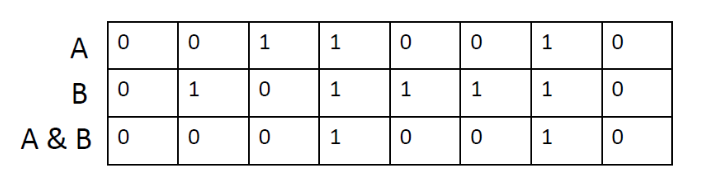
\includegraphics[scale = 0.65]{51_1.png}}                            
                        \end{center}
                        \item "Vagy" || az eredm ényben ott lesz 1 es bit, ahol valamelyik operandusban 1 es volt. Mindkét 0-nál 0 lesz.
                        \begin{center}
                            \fbox{\includegraphics[scale = 0.65]{51_2.png}}                            
                        \end{center}
                        \item "Kizáró vagy" az eredményben ott lesz 1-es bit, ahol csak egyik operandusban volt 1-es. Mindkét 0-nál és 1-nél is 0 lesz. (Elnevezése még: xor, exor, antivalencia.)
                        \begin{center}
                            \fbox{\includegraphics[scale = 0.65]{51_3.png}}                            
                        \end{center}
                    \end{itemize}
                \end{itemize}
                \textbf{Miért volt szükség logikaiműveletekre a bitműveletek mellett?}\\
                A logikai műveletek (ÉS, VAGY, XOR stb.) azért voltak szükségesek a bitműveletek mellett, mert ezekkel a műveletekkel egyszerűen és hatékonyan manipulálhatók az egyes bitek egy adott adatban. Például bitenkénti ÉS használatával egyes bitek maszkolhatók, logikai VAGY használatával bitjei beállíthatók, XOR használatával bitjei inverz állapotba hozhatók stb. Ez lehetővé teszi a hatékonyabb és precízebb adatmanipulációt.
            \end{tcolorbox}

            \begin{tcolorbox}[colback=blue!5!white,colframe=blue!50!black,title= 51. Ismertesse a C nyelv „pointer” fogalmát és az indirekció fogalmát!]
                \begin{itemize}
                    \item Annak a változónak amely nem adatot, hanem címet tárol, Pointernek nevezzük.
                    \item Az adatot pointer használatakor nem direktben érjük el (mint a sima változónál), hanem indirektben (először el kell menni a címéért). Az indirekció a jele a „ * ”.
                \end{itemize}
                \begin{center}
                    \fbox{\includegraphics[scale = 0.5]{51.png}}                            
                \end{center}
            \end{tcolorbox}

            \begin{tcolorbox}[colback=blue!5!white,colframe=blue!50!black,title= 52. Ismertesse a pointer aritmetikát!]
                \begin{itemize}
                    \item A fordító értelmez néhány műveletet a pointerekkel is.
                    \item A pointer és egy egész szám összege/különbsége: a pointer után/előtt álló adat a memóriában
                    \item Ha \(p\) egy int-re mutató pointer, \(p+1\) a következőint-re mutató pointer.
                    \item Ha \(q\) egy double-re mutató pointer, a \(q-1\) az előző double-re mutató pointer lesz.
                    \item Hasonlóan \(p+n\) az \(n.\) int-re mutató pointer lesz
                    \item Két (azonos típusú adatra mutató) pointer különbsége a köztük lévő adatok száma.
                    \item Két pointer összegenincs értelmezve, fordítási hibátokoz.
                    \item A \textbf{pre-és posztinkrementálás} és dekrementálás is értelmezett: \((++p)\) \((p++)\); utasítástól a pointer a következő/előző adatra mutat.
                    \item ha \textbf{malloc}-kal foglaltunk helyet a memóriában, nem szabad a pointert máshova állítani („elrontani”), mert a free már hibát fog okozni, mert a terület kezdetére kell mutatni a pointernek a felszabadításhoz. A hiba a programból való kilépéskor keletkezik.
                \end{itemize}
                \begin{center}
                    \fbox{\includegraphics[scale = 0.65]{52.png}}                            
                \end{center}

            \end{tcolorbox}
 
            \begin{tcolorbox}[colback=blue!5!white,colframe=blue!50!black,title= 53. Ismertesse a tömbök használatánál előforduló komplexitás-típusokat! Mondjon példát arra a műveletre{,} amelyik adott komplexitású!]
                \begin{itemize}
                    \item \textbf{Konstans:} egy elem helyének (címének) kiszámítása, elem elérése
                    \item \textbf{Lineáris:} összes elem elérése (bejárás)
                    \item \textbf{Logaritmikus:} bináris keresés.
                    \item \textbf{Polinomiális:} rendezés.
                \end{itemize}
            \end{tcolorbox}

            \begin{tcolorbox}[colback=blue!5!white,colframe=blue!50!black,title= 54. Ismertesse a tömbből való kicímzés veszélyeit!]
                \begin{itemize}
                    \item \textbf{Túlindexelés:}
                    \begin{itemize}
                        \item Ha nem ellenőrizzük a tömb határait, túlindexelhetünk, vagyis hozzáférhetünk olyan tömbelemhez, amely a tömb határain kívül esik.
                        \item Ez memóriaszivárgáshoz, adatvesztéshez vagy hibás működéshez vezethet.
                    \end{itemize}
                    \item \textbf{Alulindexelés:}
                    \begin{itemize}
                        \item Az alulindexelés esetén olyan tömbelemhez próbálunk hozzáférni, amelynek indexe negatív vagy az első elem előtti.
                        \item Ez nem várt értékekhez vagy hibás működéshez vezethet.
                    \end{itemize}
                    \item \textbf{Nem megfelelő méretű tömb használata:}
                    \begin{itemize}
                        \item Ha nem megfelelő méretű tömböt használunk a tárolandó adatokhoz, túl sok vagy túl kevés memóriát foglalhatunk le.
                        \item Ez memóriakimaradáshoz, memóriakorruptcióhoz vagy futásidejű hibákhoz vezethet.
                    \end{itemize}
                    \item \textbf{Tömb határainak átlépése:}
                    \begin{itemize}
                        \item Ha egy tömbben tárolt adatot megváltoztatunk anélkül, hogy tisztában lennénk a határaival, a változtatás más adatokat is érinthet.
                        \item Ez nem várt eredményekhez, hibás működéshez vagy adatvesztéshez vezethet.
                    \end{itemize}
                    \item \textbf{Tömbkezelési hibák:}
                    \begin{itemize}
                        \item Tömbök használatakor figyelni kell az indexelési szabályokra, a tömbméretre, az adattípusokra és az adatrendezésre.
                    \end{itemize}
                \end{itemize}
                Nem megfelelő tömbkezelés hibás működéshez, memóriaproblémákhoz vagy adatvesztéshez vezethet
            \end{tcolorbox}

            \begin{tcolorbox}[colback=blue!5!white,colframe=blue!50!black,title= 55. Ismertesse a tömbök {[ ]} operátorának jelentését! Hogy írható fel a {[ ]} operátor pointeraritmetikát felhasználva?]
                \begin{itemize}
                    \item A [ ] operátor segítségével hivatkozhatunk és manipulálhatunk egy tömb elemire. Az operátor index paramétert vár, amely megadja, hogy melyik elemre szeretnénk hivatkozni a tömbben. Az index 0-tól kezdődik, és a tömb méretével egyenlő vagy annál kisebb egész értéket vehet fel.
                    \item A [ ] operátor pointer aritmetikával is felírható. Ha XYZ egy tömbre mutató pointer, és index az elem indexe, akkor az alábbi módon használható fel a pointer aritmetika: \(XYZ[index]\) ekvivalens a \(*(XYZ + index)\) kifejezéssel.
                    \item Ez azt jelenti, hogy a [ ] operátor a \(*(XYZ+ index)\) kifejezés rövidítése, ahol XYZ a tömbre mutató pointer, és index az elem indexe. Az \((XYZ + index)\) kifejezés az XYZ címéhez hozzáadja az index értékét, majd a "*" operátorral megfelelően dereferálja azt, így elérve az adott tömb elemét.
                \end{itemize}
                Fontos megjegyezni, hogy a [ ] operátor használata a tömb méretét nem ellenőrzi, így fontos gondoskodni arról, hogy az index ne lépje túl a tömb határait.
            \end{tcolorbox}

            \begin{tcolorbox}[colback=blue!5!white,colframe=blue!50!black,title= 56. Ismertesse a szomszédcserés rendezés működését és komplexitását!]
                \begin{itemize}
                    \item A legegyszerűbb(en megírható), kis elemszámra hatékony rendezés a szomszédcserés (buborék) rendezés. Elve:
                    \begin{itemize}
                        
                        \item Összehasonlítunk két szomszédos elemet (pl. t[i]-t és t[i+1]-et).
                        \item Ha nekünk rossz sorrendben vannak, felcseréljük őket, hogy jó sorrendben legyenek.
                        \item Ha jó sorrendben vannak, nem rontjuk el őket (vagyis semmit sem csinálunk velük).
                    \end{itemize}
                \end{itemize}
                \begin{Verbatim}
procedure BubbleSort(A: array of Comparable)
n = length(A)
for i from 0 to n - 1
    swapped = false
    for j from 0 to n - i - 2
        if A[j] > A[j + 1]
            swap A[j] and A[j + 1]
            swapped = true
    end for
        if not swapped
            break
        end if
end for
end procedure                    
                \end{Verbatim}
            \end{tcolorbox}

            \begin{tcolorbox}[colback=blue!5!white,colframe=blue!50!black,title= 57. Ismertesse a függvények írásának és paraméterezésének nyelvi szabályait a C nyelvben!]
                \begin{itemize}
                    \item Minden nyelvi elemet használat előtt deklarálni kell, a változókat is, a struktúrákat is, és a függvényeket is.
                    \item Függvényen belül függvény nem definiálható (csak 1 szint létezik a memóriában).
                    \item Készíthető paraméterezett, paraméter nélküli, visszatérő érték kel rendelkező és visszatérő érték nélküli függvény. A használatkor ugyanannyi és ugyanolyan típusú változó szükséges, mint a deklarációnál. Ez alól két speciális kivétel van: a változó számú és típusú paraméterrel használható \(printf()\) és \(scanf()\). A \(va \textunderscore arg\)-ot használó függvény nem része a tematikának, ilyet nem fogunk írni.
                    \item A függvények neveire ugyanazok a megkötések, mint a változók neveire: egyedi nek kell lenni, ami nem lehet egy, már deklarált változó/függvény neve. Nem lehet foglalt kulcsszó , csak az engedélyezett karaktereket
                    \item A programunk alapértelmezetten elinduló függvénye a \(main()\) nevű, amelyet a program indításakor az operációs rendszer lefuttat. A \(main()\) átdefiniálható, mert ez csak egy cím a futtatható fájlban (exe). A return a hívóhoz tér vissza: windows-ból indítva windows-ba , visual studióból indítva oda.
                    
                \end{itemize}
                A használat meghívással valósul meg. A veremtárba elmentjük, hogy mi következik, majd a függvény memóriacímére ugrunk a memóriában a cpu végrehajtó utasítás pointerével (pl. pc-nél: IP), majd a függvény végén a veremtárból felolvasott címen (a hívás utáni címen) folytatjuk.
            \end{tcolorbox}

            \begin{tcolorbox}[colback=blue!5!white,colframe=blue!50!black,title= 58. Ismertesse a formális és aktuális paraméter fogalmát a C nyelv függvényeinél!]
                \begin{itemize}
                    \item \textbf{Formális Paraméternek:} A függvény neve utáni zárójelben a paramétereit adhatjuk meg. Minden paraméter típusát egyenként meg kell adni.
                    \item \textbf{Aktuális paraméterek:} Ezek a paraméterek az adott függvényhívás során megadott értékek vagy kifejezések. Az aktuális paraméterek a függvényhívás során átadódnak a függvénynek, és azok a formális paraméterekkel kerülnek párosításra.
                \end{itemize}
            \end{tcolorbox}

            \begin{tcolorbox}[colback=blue!5!white,colframe=blue!50!black,title= 59. Milyen paraméter-átadást használ a C nyelv?]
                A C nyelv alapértelmezetten érték szerinti paraméter-átadást használ. Ez azt jelenti, hogy amikor egy függvénynek átadunk egy paramétert, akkor a függvény a paraméter értékének másolatát kapja meg, és a függvényen belül végzett módosítások nem változtatják meg az eredeti változó értékét a hívó folyamatban.\\ \\
                \textbf{Hogy tudja megváltoztatni a függvény aparaméterei értékét úgy, hogy a hívó folyamatban is a változtatott érték szerepeljen?}\\ \\
                A C nyelvben a paraméterek értékének megváltoztatásához pointer-eket használhatunk. Azaz, ha egy függvénynek átadunk egy paramétert cím szerint ('\&' operátorral), akkor a függvényen belül közvetlenül a paraméter címére mutató pointerrel dolgozhatunk, és az értékeket közvetlenül módosíthatjuk, ami a hívó folyamatban is érvényesül.
            \end{tcolorbox}

            \begin{tcolorbox}[colback=blue!5!white,colframe=blue!50!black,title= 60. Ismertesse a lokális és globális változó fogalmakat!]
                \begin{itemize}
                    \item Minden változó, amelyet egy program blokkon \(\{\}\) belül deklaráltunk, a blokkon belül lokálisváltozóként működnek, a blokk végén \(\}\) megszűnnek. Ha még egyszer meghívjuk a függvényt, a megszűnt változót újra deklaráljuk, az előző megszűnésekor lévő érték nem lesz benne.
                    \item Azok a változók, amelyek a file szintjén (vagyis a függvényeken kívül) lettek deklarálva, globálisváltozók. Minden függvényben ugyanazt jelentik. Ha adott nevű változóból van lokális és globális is, a változó neve a lokális változót jelenti, elérakva a :: operátort a globális változót. Globális változó megadható .hfájlban is extern-ként, valamint valamelyik .c-ben (csak 1-ben) deklarálva.
                \end{itemize}
                \begin{Verbatim}
// Global variable with global scope

#include <stdio.h>

int globalVar = 10;
                    
int main() {
    // Local variable with local scope
    int localVar = 5;
}
                \end{Verbatim}
            \end{tcolorbox}

            \begin{tcolorbox}[colback=blue!5!white,colframe=blue!50!black,title= 61. Ismertesse a string tárolás C nyelvű megvalósítást{,} valamint a stringek kezelésére leggyakrabban használt függvényeket!]
            \textbf{Deklaráció és helyfoglalás:}    
                \begin{itemize}
                    \item \(char*stringnév = (char*)malloc(string mérete);\)
                    \item A mallocba nem kell \(sizeof\), mert esetünkben definició szerint 1. Kis rendszereknél, vagy nagy memóriafogyasztású programoknál ellenőrizzük a visszatérő értéket! NULL pointer esetén elfogyott a memória.
                    \item A végjel 0-nak is szüksége van helyre. Vagyis \(n\) karakter tárolásához \(n+1\) helyet kell allokálni.
                \end{itemize}
            \textbf{Stringek kezelésére leggyakrabban használt függvények:}
            \begin{itemize}
                \item \(strlen()\): String hosszának meghatározása.
                \item \(strcpy()\): String másolása.
                \item \(strcat()\): Stringek összefűzése.
                \item \(strcmp()\): Stringek összehasonlítása.
                \item \(strchr()\): Karakter keresése a stringben.
                \item \(strstr()\): String keresése a másik stringben.
            \end{itemize}
            Ezek a függvények a \(<string.h>\) könyvtárban találhatók
            \end{tcolorbox}
            
            \begin{tcolorbox}[colback=blue!5!white,colframe=blue!50!black,title= 62. Ismertesse a szöveges fájlok módosításának lépéseit!]
                \begin{itemize}
                    \item \textbf{Fájl megnyitása:} \(fopen()\) függvény (fájl megnyitása olvasásra/írásra).
                    \item \textbf{Fájl tartalmának módosítása:} \(fread()\), \(fwrite()\), \(fscanf()\), \(fprintf()\) függvények (adatok olvasása és írása a fájlba).
                    \item \textbf{Fájl bezárása:} \(fclose()\) függvény (fájl bezárása és erőforrások felszabadítása).
                \end{itemize}
                \begin{Verbatim}
#include <stdio.h>
int main() {
    
    FILE *filePointer;             

    filePointer = fopen("filename.txt", "r");               

    if (filePointer == NULL) {
        perror("Error opening file");
        return 1; // Return an error code}

        fclose(filePointer);
        return 0; // Return 0 to indicate success}                    
                \end{Verbatim}
            \end{tcolorbox}

\end{document}
                      
